Particles produced in \pp collisions traverse the detector and interact with the detector components in a characteristic manner, \eg by producing hits in the inner tracker or by initiating showers in the calorimeters. Thus, it is possible to reconstruct different objects from the detector signals, like tracks and energy deposits, and identify various types of particles which actually emerged from the collision. \\
The approach for the event reconstruction and identification of specific particles used in CMS is discussed in this chapter. First, the \textit{Particle-Flow (PF) algorithm}, used for a global description of the collision event, is introduced. Next, the reconstruction of jets is discussed in Sec.~\ref{sec:jets_reco}. In Sec.~\ref{sec:btagging} and~\ref{sec:boosted_tops}, the identification of decays from $B$ hadrons and boosted top quarks is reviewed.
\section{Global Event Description with the Particle-Flow Algorithm at CMS}
\label{sec:pf_algo}
The CMS experiment introduced the Particle-Flow algorithm~\cite{CMS-PAS-PFT-09-001} for the reconstruction of collision events which is designed to identify stable particles in an event. Types of particles which are identified by the PF algorithm are electrons and photons, charged and neutral hadrons as well as muons. In order to reconstruct the four-momenta of these particles, all sub-components of the detector are utilized. The CMS detector is very well suited for this task. The silicon tracker enclosed by the uniform magnetic field enables a very efficient track reconstruction yielding only a small track fake rate even down to small transverse momenta of $150$\mev, as discussed in Sec.~\ref{subsec:cms_tracker}. Furthermore, the strength of the magnetic field together with a high ECAL granularity allows photons to be separated from charged-particle energy deposits. \\ 
The event reconstruction starts with the identification of fundamental objects in the sub-detectors which are charged-particle tracks in the inner tracker, calorimeter clusters and muon tracks in the outer muon system. Tracks emerging from charged particles are formed following an iterative tracking algorithm~\cite{Adam:934067}. Starting from an initial seed trajectory, \eg pixel hit doublets or triplets, tracks are extrapolated to further tracker layers by taking into account multiple scattering and energy loss in the material. Each iteration proceeds with a removal of unambiguously allocated hits from the previous iteration. \\
Furthermore, calorimeter clusters are formed based on adjacent calorimeter cells in each sub-detector separately: ECAL barrel, ECAL endcap, HCAL barrel, HCAL endcap, PS first layer and PS second layer. First, seed clusters are defined as local calorimeter-cell energy maxima. Second, neighbouring cells are combined with seed clusters when their energy exceeds a pre-defined threshold representing two standard deviations of the electronics noise. In the HF however, no clustering is performed and each calorimeter cell gives rise to one cluster. \\
A particle traversing the detector gives typically rise to several of such elementary objects: one charged-particle track, and/or several calorimeter clusters and/or one muon track. Consequently, a dedicated link algorithm is applied in order to connect these elements. Linked elements form blocks and remove a potential double-counting of the same object in different detector parts. First, charged-tracks are associated to calorimeter clusters if the extrapolated trajectory matches the cluster within the cluster boundaries. This is done considering effects like gaps and cracks between detector components, uncertainty on the shower position or multiple scattering. To account for bremsstrahlung, also tangents of the tracks are extrapolated to the respective energy clusters. In addition, also ECAL and HCAL clusters can be connected to each other by linking clusters in the more granular calorimeter to clusters in the less granular one. Finally, global muons can be defined by associating charged-tracks from the tracker with muon tracks reconstructed in the muon system. \\
After the identification of such blocks of elements, the PF algorithm creates a list of all particles contained in the event applying dedicated quality criteria interpreting the blocks in terms of particles. The identification of muons and a removal of their tracks from the blocks is followed by an assignment of electrons and associated bremsstrahlung from tracks and linked ECAL clusters. After these have been removed from the list of blocks as well, remaining blocks with a good quality track are considered to be charged hadrons. Their momenta are determined from combining the track momentum and the respective energy in the calorimeter cluster. If the cluster energy exceeds the measured momentum from the track beyond the expected calorimeter energy resolution, it constitutes a photon and if the excess is larger than the total ECAL energy also a neutral hadron. Finally, remaining ECAL and HCAL clusters not linked to any track give rise to photons and neutral hadrons. \\
The complete set of particles can then be used to derive further objects and quantities, like jets as discussed in Sec.~\ref{sec:jets_reco}, missing transverse energy \met or decay products of tau leptons. More detailed information on the specific quality criteria required for the identification of certain particles is given in Chap.~\ref{chap:Resolution},~\ref{chap:RA2} and~\ref{chap:Stop} for each analysis presented in this thesis.

\section{Reconstruction of Jets}
\label{sec:jets_reco}
As stated earlier, the searches for supersymmetry presented in this thesis are performed in final states containing missing transverse energy and several jets. % jets are the experimental signatures of quarks and gluons and constitute of a collimated spray of hadrons. 
In order to identify a particular jet and relate its properties to the original parton, a proper jet definition is needed. Typically, a \textit{jet algorithm} determines how to cluster particles into a jet. Furthermore, it has to be defined how to assign a momentum to the jet. At CMS, the standard procedure is to assign the four-momentum sum of all jet constituents to the jet. 
%Different jet algorithms are introduced in Sec.~\ref{subsec:jets_algos} followed by a discussion of different jet types used at CMS in Sec.~\ref{subsec:jets_types}. The jet transverse-momentum response is defined in Sec.~\ref{subsec:jets_response} and the calibration of jet energies is reviewed in Sec.~\ref{subsec:jets_calib}.
\subsection{Jet Algorithms}
\label{subsec:jets_algos}
\begin{figure}[!tp]
  \centering 
  \begin{tabular}{c}
  %  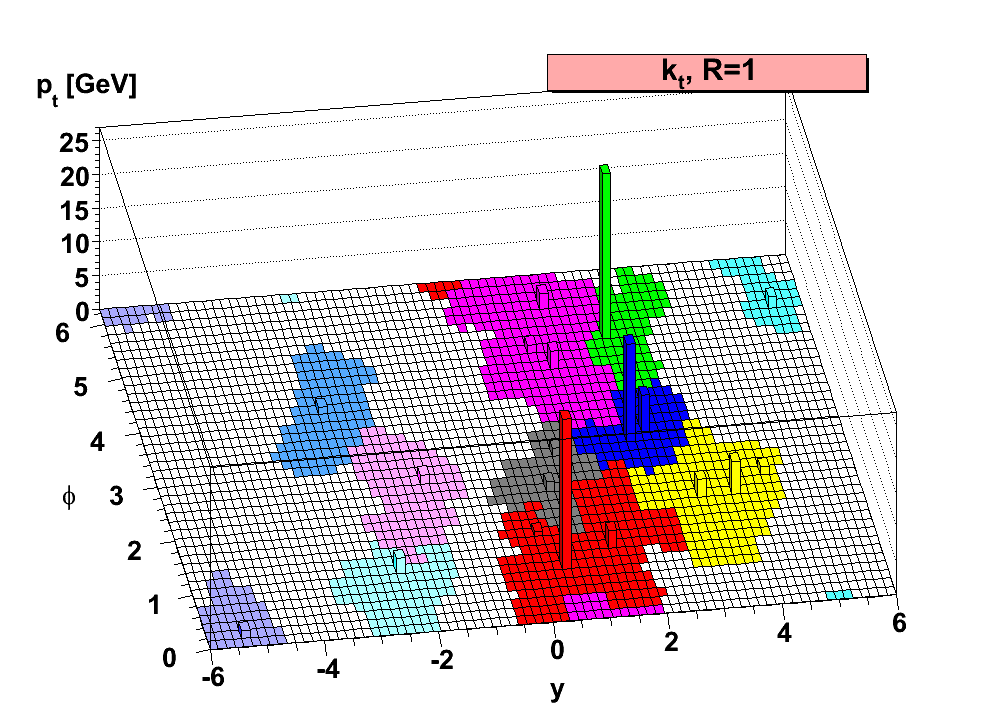
\includegraphics[width=0.49\textwidth]{figures/herwig-parton-level-ev-kt.png} &
  %  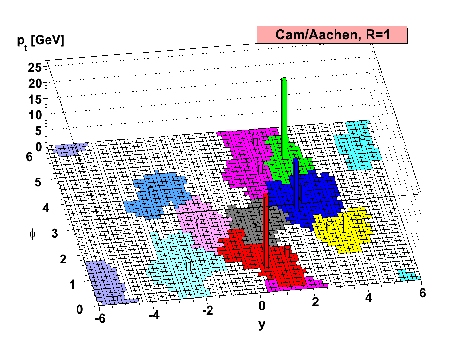
\includegraphics[width=0.49\textwidth]{figures/herwig-parton-level-ev-cam.png} \\
  %  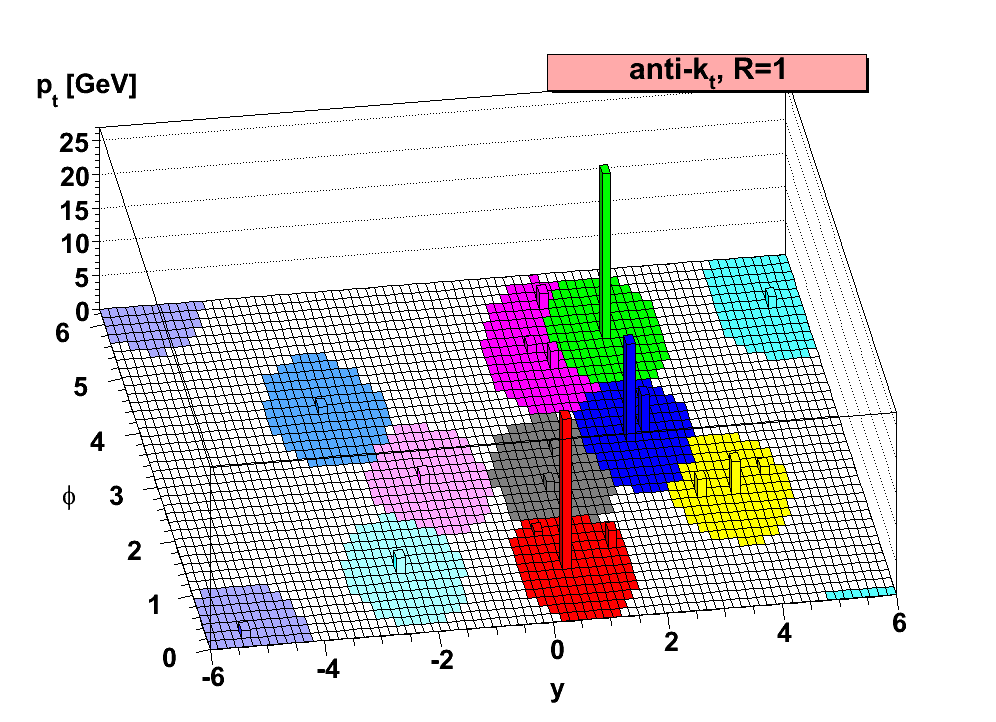
\includegraphics[width=0.49\textwidth]{figures/herwig-parton-level-ev-antikt.png} &
  %  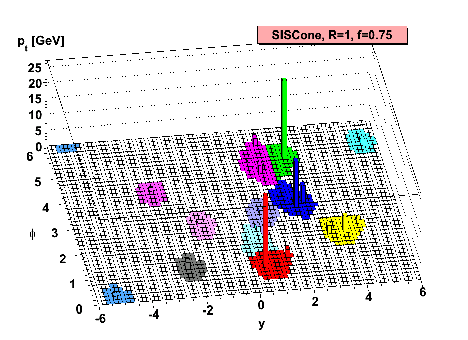
\includegraphics[width=0.49\textwidth]{figures/herwig-parton-level-ev-siscone.png}  
    \includegraphics[width=1.0\textwidth]{figures/JetAlgos.pdf} 
  \end{tabular}
  \caption{Example parton-level event generated with \herwig, adding many random soft particles, that is clustered with the $k_\mathrm{T}$ algorithm (\textit{top left}), the CA algorithm (\textit{top right}), the SISCone algorithm (\textit{bottom left}) and the anti-$k_\mathrm{T}$ algorithm (\textit{bottom right}). Colours illustrate all particles clustered to the resulting hard jets~\cite{Salam:2009jx}.}
  \label{fig:jet_algos}
\end{figure}
A jet algorithm usually provides a prescription how to combine individual particles into a single jet based on some distance criterion. Good jet algorithms though should be able to identify jets that are neither sensitive to the emission of soft particles (\textit{infrared safety}) nor to the collinear splitting of particles (\textit{collinear safety}). These features named \textit{IRC safety} are desirable as calculations in QCD perturbation theory rely on the cancellation of divergences related to IRC processes. Thus, if jets are sensitive to such effects, cancellations are not ensured and cross sections calculated at fixed order perturbation theory would diverge. \\
An introduction to the most commonly used jet algorithms known as \textit{cone algorithms} and \textit{sequential recombination algorithms} is given. A comprehensive overview of jet algorithms and properties can be found for instance in~\cite{Salam:2009jx}. Technical implementations of various jet algorithms are provided by the \textit{FastJet} package~\cite{Cacciari:2011ma, Cacciari:2005hq}.
\ \\
\begin{description}
 \item \textbf{Cone Algorithms:} Cone algorithms are based on the general idea that the main kinematics in an event are not changed by specific effects from hadronisation and thus a jet is defined by a set of particles within a stable cone around their centre of mass. Typically, separate angular or energy parameters are used to perform the jet finding. A very common approach is implemented in \textit{iterative cone} (IC) algorithms. Here, a seed constituent $i$, which is for instance the constituent with the highest transverse momentum, defines the initial direction. Then, momenta of all constituents $j$ within a cone defined by
\begin{equation}
 \Delta R_{i,j}^2 < R^2
\end{equation}
are added to the momentum of the seed, with $\Delta R_{i,j}$ calculated as introduced in Sec.~\ref{subsec:cms_coordinates}. The resulting direction is used as new seed direction and the whole procedure is repeated until a stable cone is achieved. The dimensionless parameter $R$ hence defines the jet radius. After finding such a jet, all constituents are removed from the input list and further jets are clustered from the remaining objects. This progressive removal approach avoids to form jets with overlapping cones. However, such a procedure is not IRC safe as collinear splittings can lead to varying seeds in the event and thus to different final ensembles of jets. \\
However, cone algorithms are IRC safe when instead of iteratively forming stable cones all stable cone solutions are identified at once. This procedure is denoted \textit{seedless cone} (SC) algorithm. The usage of such algorithms though is typically impractical as the computation time increases exponentially with the number of particles to be considered so that even for 100 particles it is not solveable at any reasonable timescale. A feasible implementation of a seedless cone algorithm featuring an $\mathcal{O}(N \, \mathrm{log} (N))$ time-dependence is given by the SISCone algorithm~\cite{Salam:2007xv}. As it is usually nonetheless still more time consuming than sequential algorithms, as described in the next part, the SISCone algorithm is not used by CMS.
 \item \textbf{Sequential Recombination Algorithms:} The basic concept of sequential clustering algorithms is to iteratively group pairs of particles together based on some distance measure and thus, to some extent, reconstruct the evolution of a parton shower. At hadron colliders where the total energy of a collision is unknown, a suitable metric based on variables invariant under longitudinal boosts is 
\begin{equation*}
d_{ij} = \mathrm{min}(k_\mathrm{T,i}^{2p}, k_\mathrm{T,j}^{2p}) \frac{\Delta R_{ij}^2}{R^2}
\end{equation*}
\begin{equation*}
d_{iB} = k_\mathrm{T,i}^{2p}
\end{equation*}
with the distance $d_{ij}$ between final state objects $i$ and $j$ carrying transverse momentum $k_\mathrm{T}$ and the distance of the object to the beam $d_{iB}$. While $\Delta R_{ij}$ denotes the spatial separation in the $(\eta, \phi)$-plane, $R$ and $p$ are free parameters of the algorithm. The recombination is done by first calculating $d_{ij}$ and $d_{iB}$ for all objects in the final state and then identifying the minimum value. If the minimum is $d_{ij}$, the two objects $i$ and $j$ are combined, \ie their four-momenta are added to form one new object. Afterwards distances are computed again. However, if the minimum is $d_{iB}$, object $i$ is declared a jet and removed from the input list. This procedure is repeated until all objects are assigned. In this context, the parameter $R$ acts as an angular cut-off and thus has a similar role as the jet radius in cone algorithms. \\
Depending on the choice of the parameter $p$, different types of algorithms are distinguished which are all IRC safe. An illustration of an arbitrary example event, where jets are clustered with the different jet algorithms, is shown in Fig.~\ref{fig:jet_algos}. The $k_T$ \textit{algorithm} uses $p = 1$~\cite{PhysRevD.48.3160} and thus clusters soft particles first. This results mainly in irregularly shaped jets (\cf Fig.~\ref{fig:jet_algos}) and makes them sensitive to radiation in the event. Consequently, they are difficult to calibrate and therefore impractical to use at hadron colliders. The \textit{Cambridge-Aachen algorithm} or short \textit{CA algorithm}~\cite{Dokshitzer:1997in, Wobisch:1998wt} utilizes $p = 0$. Thus, it does not rely on momentum information, but clusters jets based on the angular separation of input objects. This allows a direct geometric interpretation of jets and has been proven to be a jet algorithm especially suited for analyses of jet substructure as will be discussed later in Sec.~\ref{sec:boosted_tops}. These jets still reflect the structure of the parton shower, but are less affected by soft radiation than the $k_\mathrm{T}$ algorithm. Finally, the \textit{anti-$k_T$ algorithm} uses $p = -1$~\cite{1126-6708-2008-04-063} and starts the jet clustering beginning with the hardest objects in the event. Hence, the evolution of the parton shower is not reproduced. The anti-$k_\mathrm{T}$ algorithm tends to form very regular shaped jets as the four-momentum of the core of the jet is not much affected by the softer components which are clustered later in the process. Typically, the regular shape allows an easier calibration of anti-$k_\mathrm{T}$ jets than, \eg of $k_\mathrm{T}$ jets. 
\end{description}

\subsection{Jet Types at CMS}
\label{subsec:jets_types}
The default jets used at the CMS experiment are jets clustered by the anti-$k_\mathrm{T}$ algorithm using a distance parameter of $R = 0.5$ (AK5 jets). This algorithm can be applied to reconstructed detector signals resulting in \textit{detector-level} jets or to final-state particles after hadronisation and decay, in simulated events, giving rise to \textit{particle-level} jets.  \\
Based on the information used from the various CMS subdetectors for the jet clustering, different types of detector-level jets are distinguished~\cite{1748-0221-6-11-P11002}:
\begin{figure}[!tp]
  \centering 
  \begin{tabular}{c}
    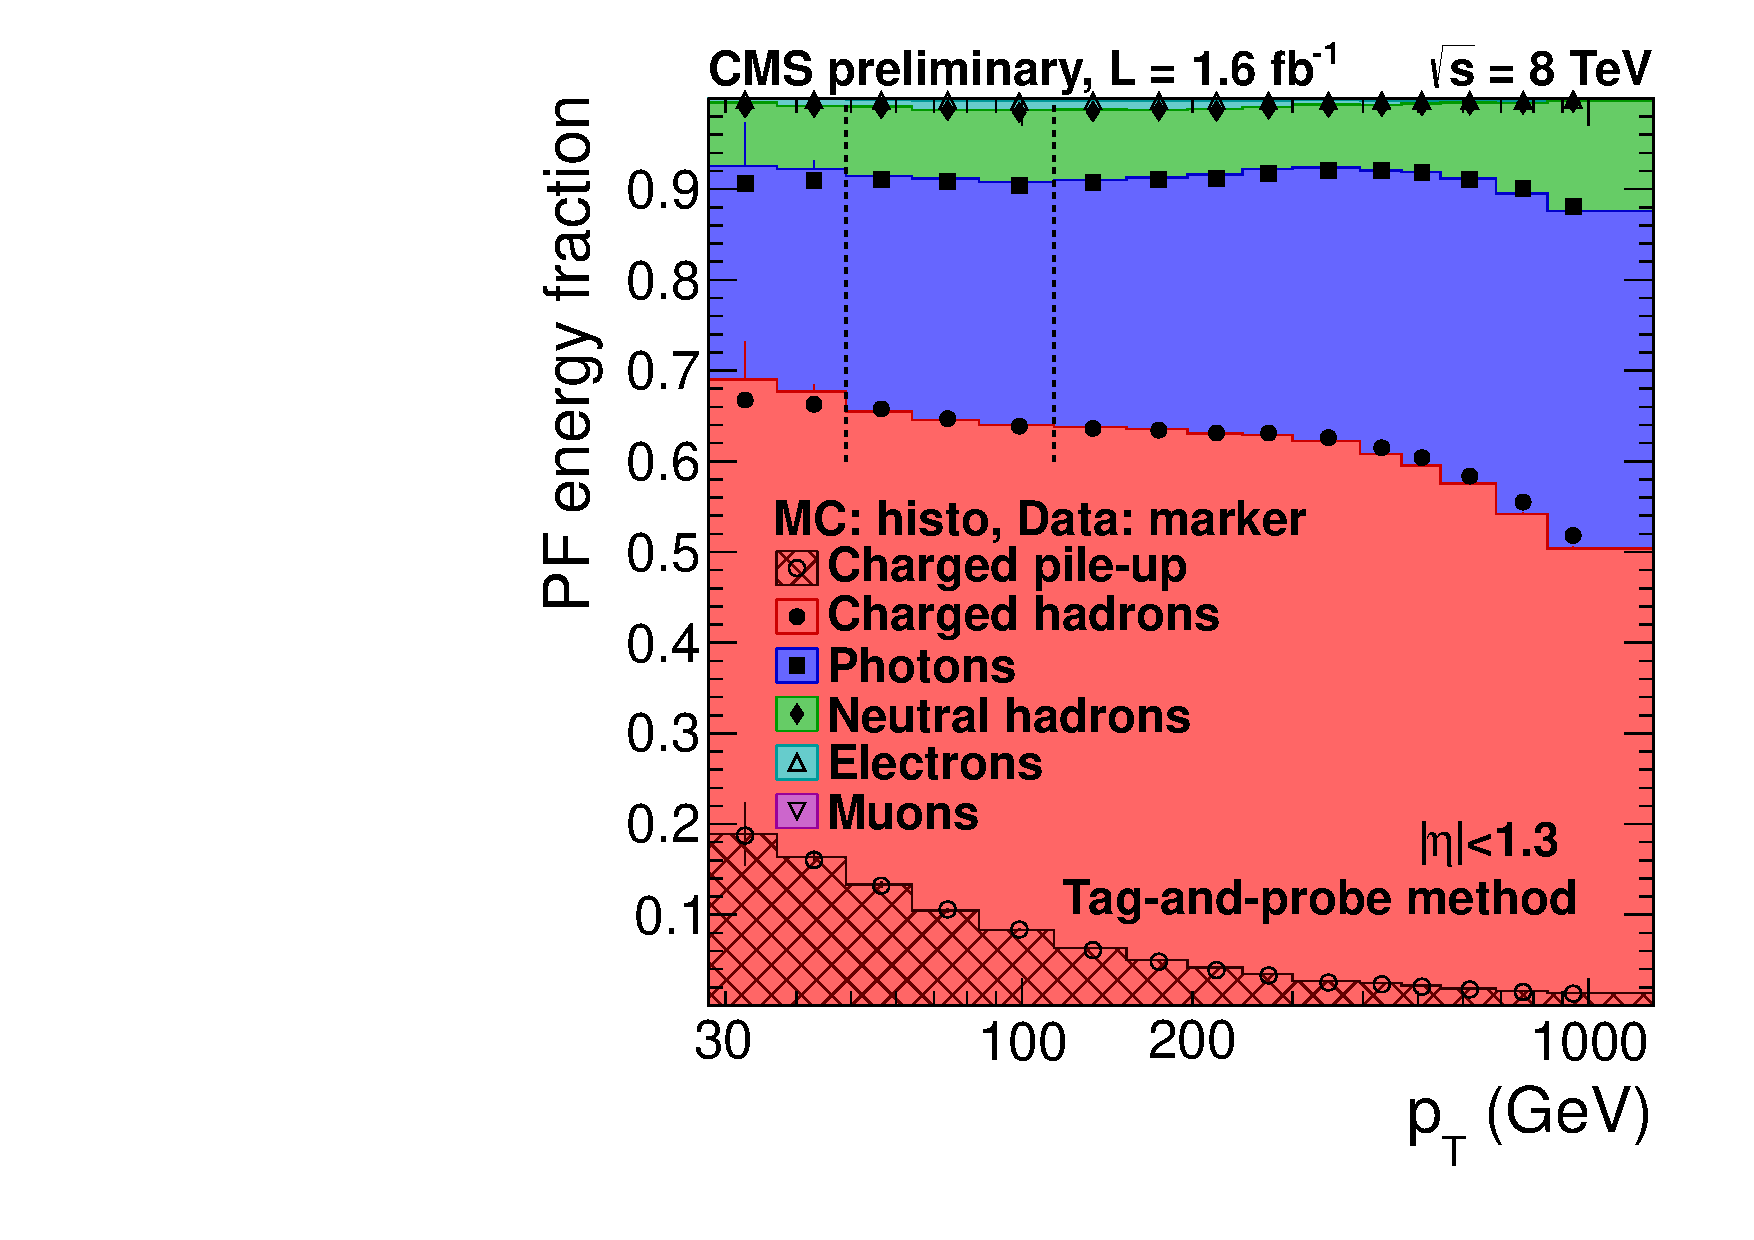
\includegraphics[width=0.7\textwidth]{figures/calcFrac_Frac0_MC-1.pdf} 
  \end{tabular}
  \caption{Composition of the PF jet energy versus jet \pt in the barrel detector region $|\eta| < 1.3$ in simulated events (coloured histograms) and data (solid markers)~\cite{CMS-DP-2012-012}.}
  \label{fig:jets_pf_comp}
\end{figure}
\begin{description}
 \item \textbf{Calorimeter (Calo) jets:} Calo jets are clustered from energy deposits in the calorimeters. For this purpose, calorimeter towers are defined which consist of at least one HCAL cell and the geometrically associated ECAL cells. For instance in case of the barrel detector region, a calorimeter tower consists of one HCAL cell and $\mathrm{5 \times 5}$ ECAL cells. The four-momentum of each tower is defined by the tower position as seen from the primary interaction vertex and the energy deposit in the tower above a certain threshold assuming a mass of zero. 
 \item \textbf{Jet-Plus-Track (JPT) jets:} JPT jets are reconstructed from calorimeter jets complemented by tracking information~\cite{CMS-PAS-JME-09-002}. Tracks of charged particles can be associated to calo jets based on the separation of the jet axis and the momentum vector of the track in the $(\eta,\phi)$-plane. Associated tracks are projected to the jet cone and are exploited to correct the jet energy and direction. 
 \item \textbf{Particle-Flow (PF) jets:} PF jets are clustered from the four-momentum vectors of Particle-Flow candidates as identified by the PF algorithm described in Sec.~\ref{sec:pf_algo}. Typically, these types of jets show the best performance as the excellent resolution of the tracking system and the ECAL are utilized. Only neutral hadrons which constitute around 15\% of the jet energy (cf. Fig.~\ref{fig:jets_pf_comp}) rely on the energy measurement of the HCAL with its relatively poor resolution. Thus, PF jets are the default jets to be used at the CMS experiment as it is done within this thesis. In order to mitigate influences from pileup, charged hadrons unambigously associated to vertices other than the primary vertex can be removed from the jet algorithm input list before the actual jet clustering is performed. This technique is referred to as \textit{charged-hadron subtraction} (CHS) and used as default throughout this thesis. The respective jets are denoted PFCHS jets.
\end{description}

\subsection{Jet Transverse-Momentum Response}
\label{subsec:jets_response}
In general, the jet transverse momentum as measured at detector level is not necessarily equal to the energy of the original particle. This effect is quantified by the \textit{jet transverse-momentum response} $\mathcal{R}$ which is defined as 
\begin{equation}
  \mathcal{R} = \frac{\pt}{\pt^{\mathrm{particle}}} 
  \label{eq:response}
 \end{equation}
with the transverse momentum \pt of the jet measured at detector level and the transverse momentum $\pt^{\rm{particle}}$ of the original particle-level jet. Thus, the jet response provides a measure of the jet momentum visible in the detector compared to the actual momentum of the particle after hadronisation and decay. \\
The jet response usually depends on the jet momentum as well as on the pseudorapidity which is expected since the precision of the jet measurement is directly related to the energy of the particles and the resolution of the detector sub-components. This is for instance caused by the non-linear response of the calorimeters, the specific track-reconstruction efficiency, the individual amount of detector material, cracks in the detector layout or different instrumentation. \\
In this thesis, the average response $\langle \mathcal{R} \rangle$ is referred to as \textit{jet energy scale} (JES) while the width of the response distribution is denoted as relative \textit{jet transverse-momentum resolution} (JER).
\ \\
\subsection{Jet Energy Calibration}
\label{subsec:jets_calib} 
\begin{figure}[!t]
  \centering 
  \begin{tabular}{c}
    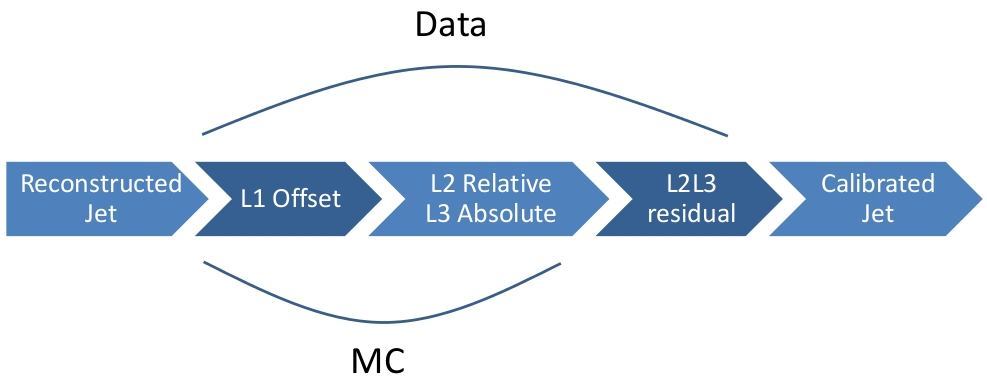
\includegraphics[width=0.95\textwidth]{figures/JEC.jpg} 
  \end{tabular}
  \caption{Sketch of the factorized approach used for jet energy corrections at the CMS experiment.}
  \label{fig:jec_sketch}
\end{figure}
In order to relate the measured jet momentum on average to the momentum of the corresponding particle-level jet, a jet calibration procedure is applied. This compensates for the non-linear response of the calorimeters and ensures that $\langle \mathcal{R} \rangle = 1$. Within the CMS experiment, a factorized approach is utilized which is described in detail in~\cite{1748-0221-6-11-P11002} and illustrated in Fig.~\ref{fig:jec_sketch}. The actual set of correction factors used in this thesis, if not stated otherwise, is documented in~\cite{CMS-DP-2013-033}. \\
The calibrated jet four-momentum vector $p^\mathrm{cor}$ is obtained from the raw jet four-momentum vector $p^\mathrm{raw}$ by scaling the raw momentum with a correction factor $C$ according to
\begin{equation}
p^\mathrm{cor} = C \cdot p^\mathrm{raw} = C_{\mathrm{offset}}(\pt^\mathrm{raw}, \eta) \cdot C_{\mathrm{rel}}(\eta) \cdot C_{\mathrm{abs}}(\pt') \cdot C_\mathrm{res}(\pt'', \eta) \cdot p^\mathrm{raw}
\end{equation} 
 where $C$ is composed of the offset correction $C_{\mathrm{offset}}$, the calibration factors $C_{\mathrm{rel}}$ and $C_{\mathrm{abs}}$ as well as residual correction factors $C_{\mathrm{res}}$. While $C_{\mathrm{offset}}$, $C_{\mathrm{rel}}$ and $C_{\mathrm{abs}}$ are applied to both data and simulation, the residual correction factors $C_{\mathrm{res}}$ are applied to data only. Each correction factor is applied sequentially after the other in a fixed order such that $\pt'$ denotes the transverse momentum after the application of the offset correction and $\pt''$ is the transverse momentum after applying the respective previous corrections. Some details for each individual correction are given in the following: 
\begin{description}
 \item \textbf{L1 Offset:} The L1 offset correction is designed to compensate for additional energy contributions arising from instrumental noise or pileup events. The \pt offset is estimated in dependence of $\eta$, the effective jet area $A_j$ and the \pt-density $\rho$ (\textit{hybrid jet area method}~\cite{Cacciari2008119}). \\
The jet area is determined by adding a large number of inifinitely soft four-momentum vectors to the event. The active jet area is then defined as the fraction of soft particles clustered together with the true hard jet components. The \pt-density $\rho$ is defined on an event-by-event basis as the median of the distribution $\pt^{j}/A_{j}$ where $j$ denotes all reconstructed jets in the event. The estimated offset in simulated QCD multijet events and data is illustrated in Fig.~\ref{fig:l1offset}.
\begin{figure}[!h]
  \centering 
  \begin{tabular}{c}
    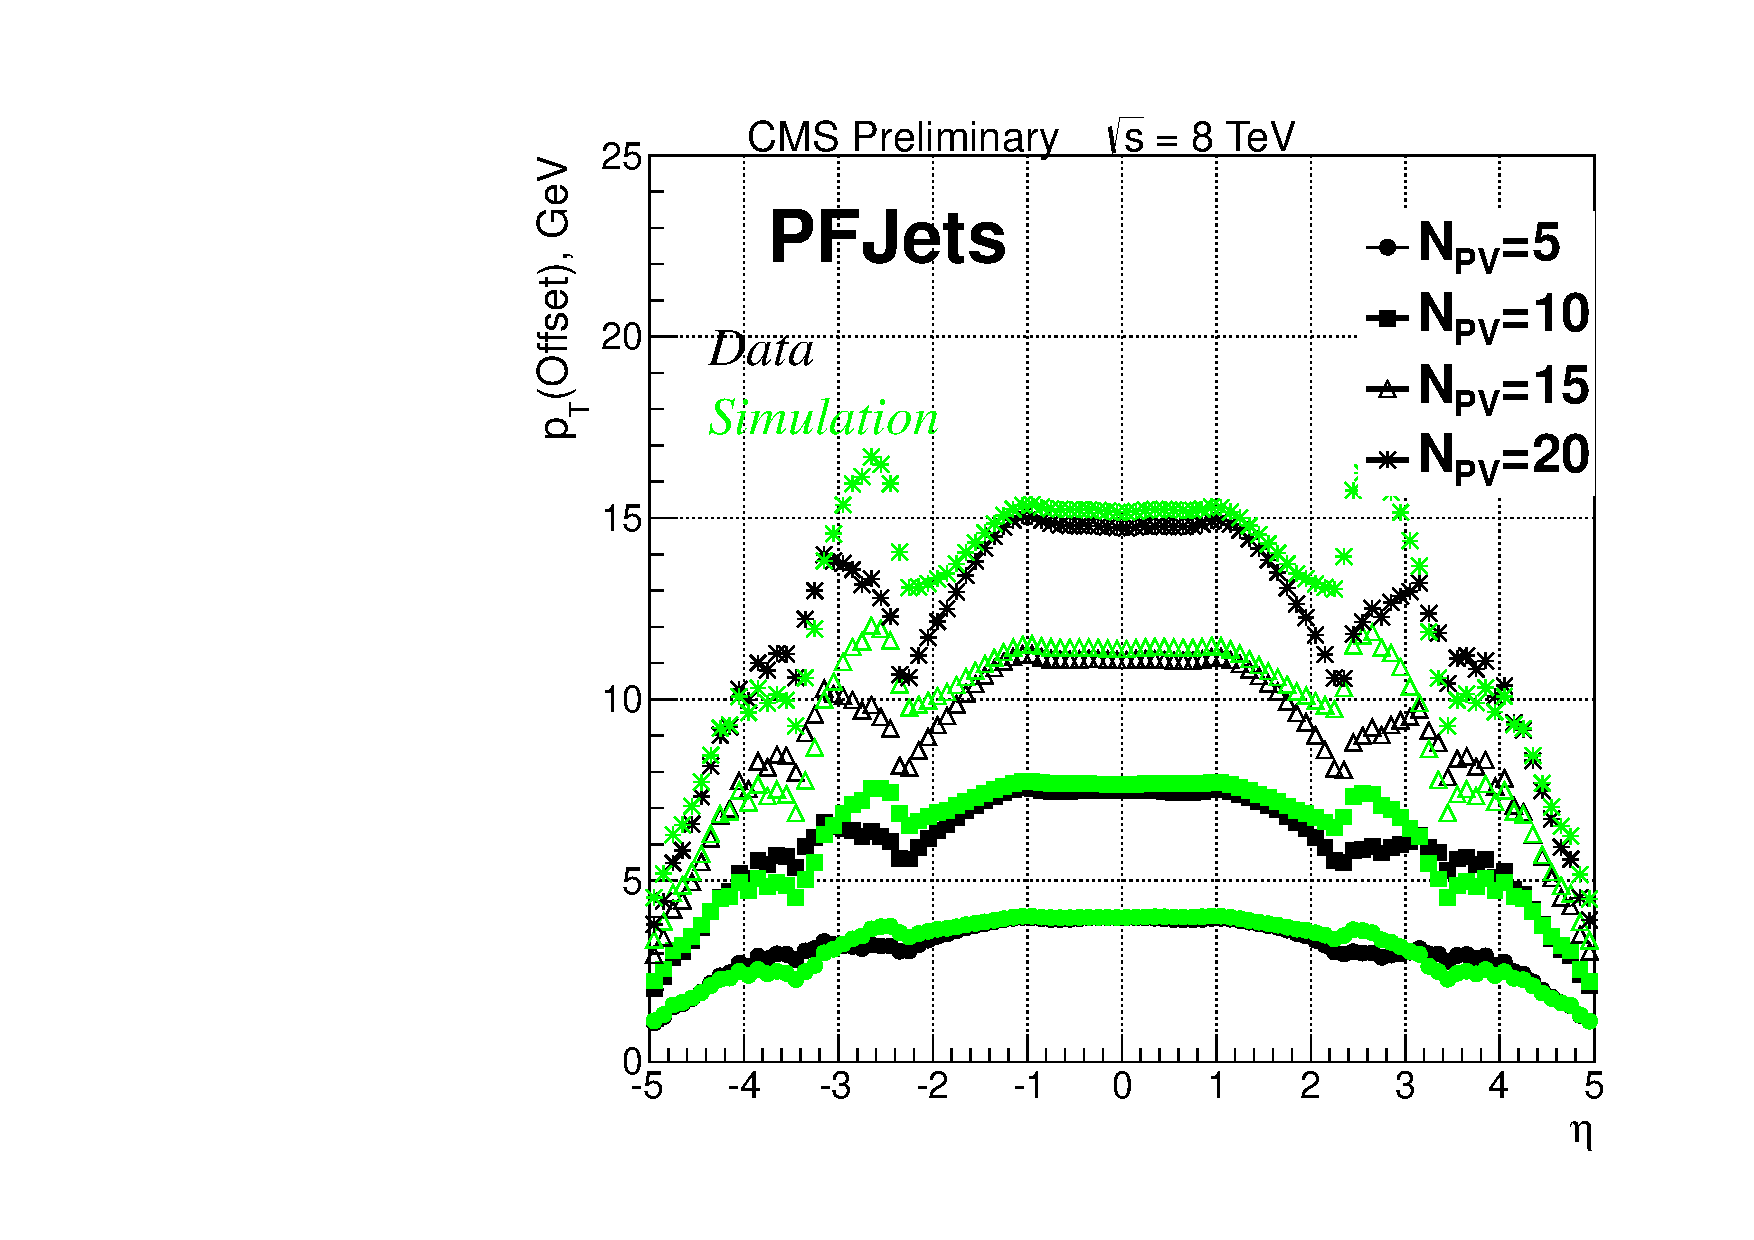
\includegraphics[width=0.51\textwidth]{figures/OffsetVsEta_NPV_PF5_data53_vs_mc53.pdf} 
  \end{tabular}
  \caption{L1 offset transverse momentum correction for AK5 PF jets as a function of jet pseudorapidity in data (black) and simulation (green). Different intervals of reconstructed primary vertices ($\mathrm{N_{PV}}$) are shown with different markers~\cite{CMS-DP-2013-033}.}
  \label{fig:l1offset}
\end{figure}
 \item \textbf{L2 Relative $+$ L3 Absolute Correction:} The L2 relative correction is designed to make the jet energy scale uniform with respect to $\eta$ while the L3 absolute correction ensures a uniform response versus \pt. Both corrections are entirely estimated from simulated QCD multijet events. The correction is defined as the inverse of the average response $1/\langle R \rangle$ at fixed $\pt^\mathrm{gen}$ and illustrated in Fig.~\ref{fig:l2l3}.
\begin{figure}[!h]
  \centering 
  \begin{tabular}{c}
    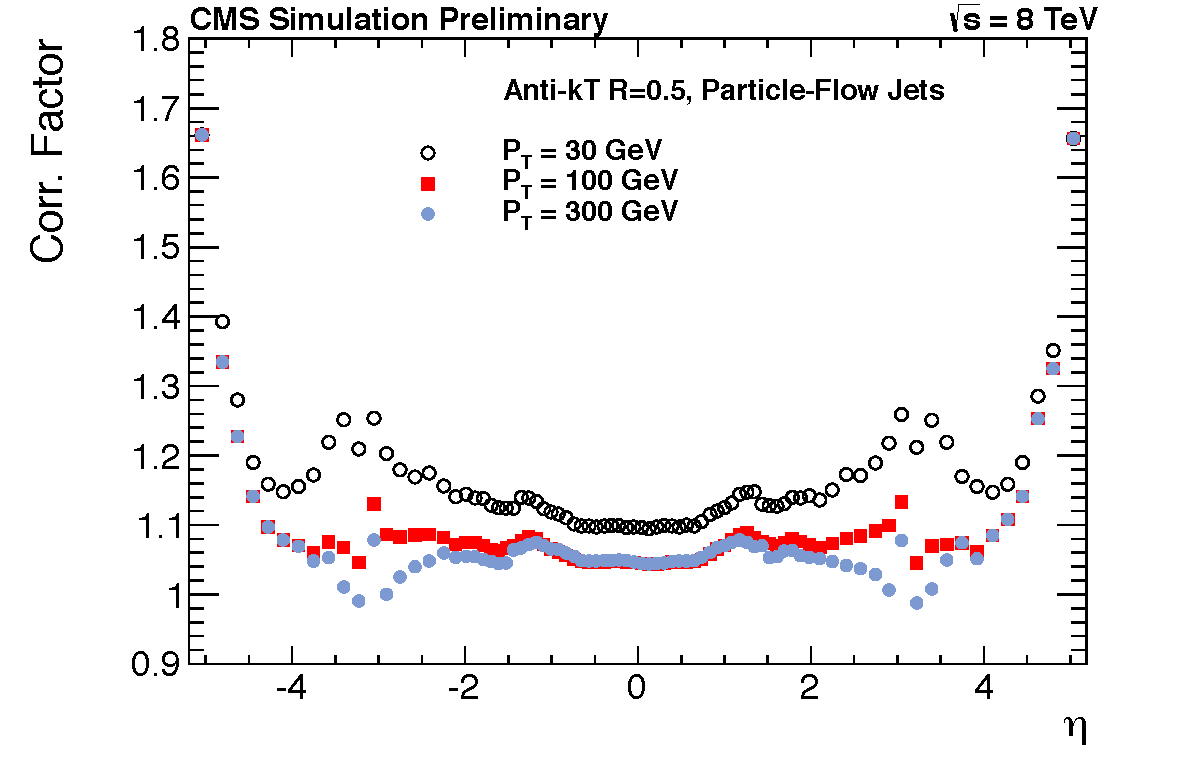
\includegraphics[width=0.7\textwidth]{figures/CorrectionVsEta_Overview_TDR_ak5pfl1_L2L3.pdf} 
  \end{tabular}
  \caption{MC-Truth corrections for AK5 PF jets as a function of jet pseudorapidity for three reference transverse momentum values: 30\gev (white hollow circles), 100\gev (red squares) and 300\gev (blue circles)~\cite{CMS-DP-2013-033}.}
  \label{fig:l2l3}
\end{figure}
 \item \textbf{L2L3 Residual Correction:} In order to compensate for remaining response differences between simulated events and data, residual correction factors are derived. These are applied to data only and correct for remaining differences in the data-to-simulation ratio of the relative jet energy scale. Residual corrections can be derived from events that have momentum balance in the transverse plane, like dijet events (used for the determination of the L2 residual correction) or $\mathrm{Z/\gamma+jet}$ events (used for the measurement of the L3 residual correction). The L2 residual correction is illustrated in Fig.~\ref{fig:l2res}.
\begin{figure}[!h]
  \centering 
  \begin{tabular}{c}
    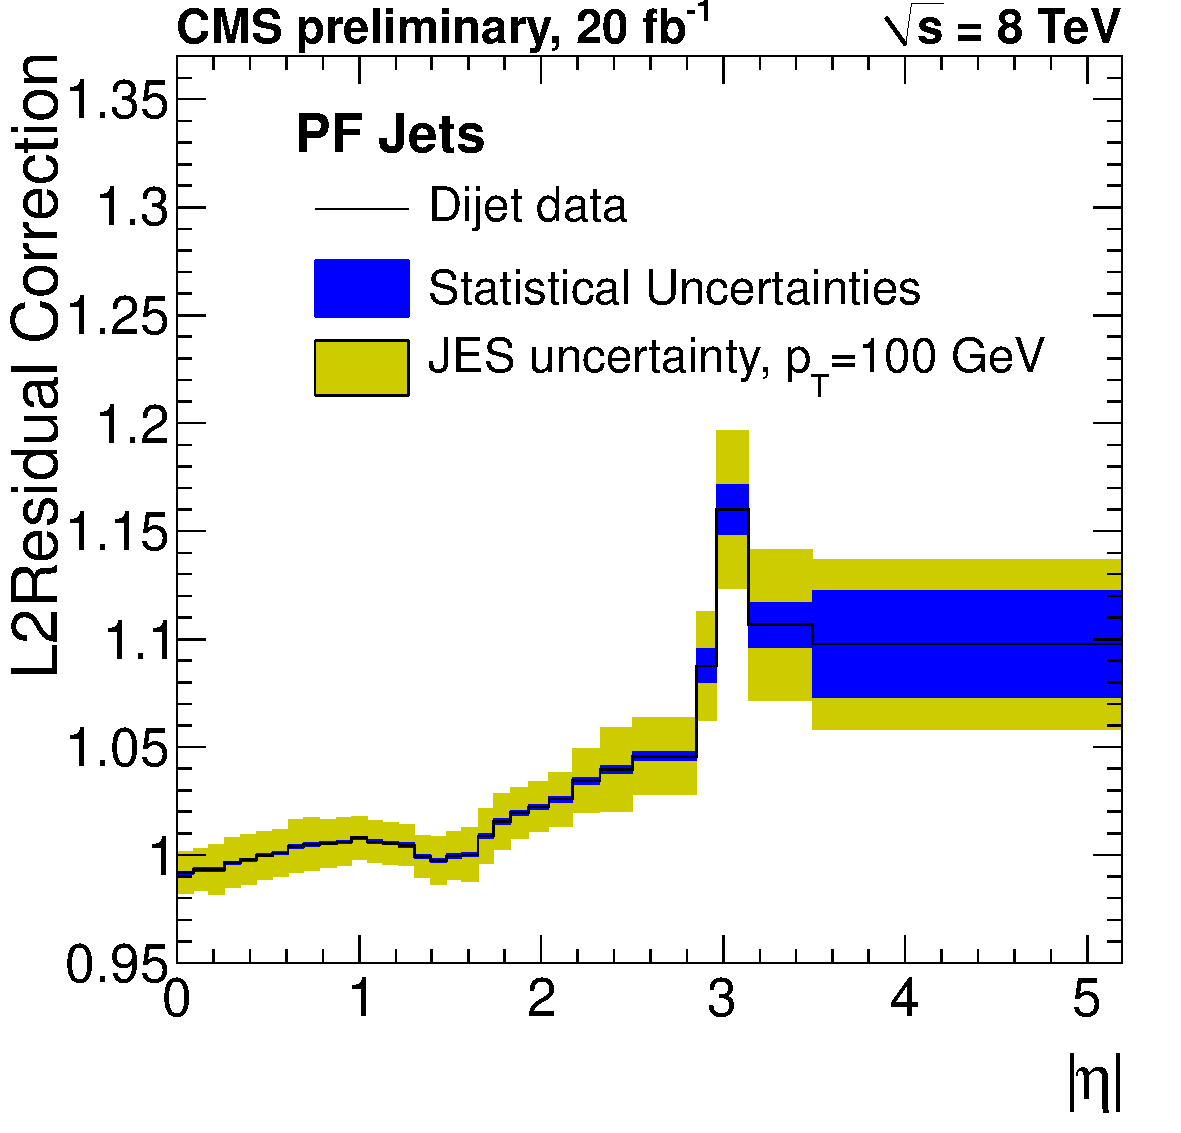
\includegraphics[width=0.51\textwidth]{figures/ResComp_FSRcorr_residuals_Abseta_PF_DiJetData.pdf} 
  \end{tabular}
  \caption{L2 residual corrections for AK5 PF jets as a function of jet pseudorapidity, obtained from dijet events, shown with JES uncertainty (yellow band) and the statistical uncertainty (blue band)~\cite{CMS-DP-2013-033}.}
  \label{fig:l2res}
\end{figure}

\end{description}
The calibration factors are obtained with respect to the average flavour composition of a QCD mulitjet sample. Thus, further steps of correction factors can be applied for specific analysis purposes, \eg correcting the different response for various jet flavours. However, such higher order corrections are not used in this thesis.  
% and illustrated in Fig. ... \todo{Fig. JEC}. In total, the size of the JES corrections are at the order of ... \todo{size of JEC}.

\section{Identification of b-Quark Jets}
\label{sec:btagging}
Jets arising from the hadronization of bottom quarks are usually referred to as \textit{b jets}. As these are present in many physics processes, \eg the decay of top quarks, it is crucial to identify b jets, \ie distinguish them from jets initiated by gluons or light-flavour quarks. Typically, the identification of b jets is denoted \textit{b tagging} which exploits the distinct properties of b quarks for the identification of the respective jets. In general, $B$ hadrons have a lifetime of around $c\tau \approx 500$\,\textmu m, so that they travel in the detector before they actually decay. This results typically in a measurable secondary vertex that is displaced with respect to the primary interaction. Furthermore, b-quark jets feature a high number of charged particles per decay, resulting in jets with several tracks, and often exhibit soft leptons emerging from semi-leptonic decays of $B$ mesons. \\
The CMS experiment exploits the specific b-jet properties in dedicated b-tagging algorithms for an efficient b-jet identification. Each algorithm determines a discriminator value per jet indicating how b-jet-like a jet behaves. Based on that, working points are defined corresponding to a specific minimum threshold of the discriminator value. These working points are named \textit{loose}, \textit{medium} and \textit{tight} and correspond to a misidentification probability, \ie the probability to identify a non-b jet as b jet, of $10\%$, $1\%$ and $0.1\%$ for an average jet transverse momentum of $80$\gev, respectively. B-tagging algorithms comissioned within the CMS experiment are~\cite{Chatrchyan:2012jua}:
\begin{description}
 \item \textbf{Track Counting (TC) algorithm:} A powerful discriminator for the decay products of a $B$ hadron from prompt tracks is the \textit{impact parameter} (IP) of a track with respect to the primary vertex. Its significance can be computed by taking the ratio of the IP to its respective uncertainty. Tracks in a jet are sorted by decreasing values of the IP significance by the TC algorithm. Depending on whether the IP significance of the second or the third ranked track is chosen as discriminator, the algorithm is denoted \textit{Track Counting High Efficiency} (TCHE) or \textit{Track Counting High Purity} (TCHP) algorithm. 
 \item \textbf{Jet Probability (JP) algorithm:} The JP algorithm extends the simple TC algorithm by connecting the information about the IP from a couple of tracks in the jet. A likelihood is calculated that all tracks of the jet stem actually from the primary vertex. This approach can be varied by giving more weight to tracks with the highest IP significance. The maximum of such tracks is four and matches the average number of reconstructed charged particles from the decay of $B$ hadrons. This version is called \textit{Jet B Probability} (JBP) algorithm.
 \item \textbf{Simple Secondary Vertex (SSV) algorithm:} A further useful discriminating feature for b tagging is the presence of a secondary vertex and related kinematic variables, like the flight distance and direction, which can be determined from the vector between the primary and secondary vertex. The SSV exploits the significance of the flight distance which is given by the flight distance divided by the associated uncertainty. Two different versions of this algorithm exist targeting on the one hand a \textit{High Efficiency} (SSVHE) and on the other hand a \textit{High Purity} (SSVHP). The SSVHE is based on vertices with at least two associated tracks, while the SSVHP uses vertices with at least three tracks. Typically, the efficiency of the algorithm is limited by the reconstruction efficiency of secondary vertices which is at the order of 65\%.   
 \item \textbf{Combined Secondary Vertex (CSV) algorithm:} The CSV algorithm utilizes an approach combining information from secondary vertices as well as track-based lifetime information and thus is able to exceed the efficiency of SSV algorithms. It allows an efficient identification of b jets, also in cases where no secondary vertex can be reconstructed. Often, pseudo-vertices can be formed from tracks even when failing the reconstruction of an actual secondary vertex which allows to derive some secondary vertex related quantities. Important variables used in the CSV algorithm are the flight distance significance, vertex mass, number of tracks at the vertex, number of tracks in the jet and the IP sigificances for the tracks in the jet. These variables are used to compute two likelihood ratios which can be used to distinguish either c and b jets or light-parton and b jets. 
\end{description}  
\begin{figure}[!tp]
  \centering 
  \begin{tabular}{cc}
    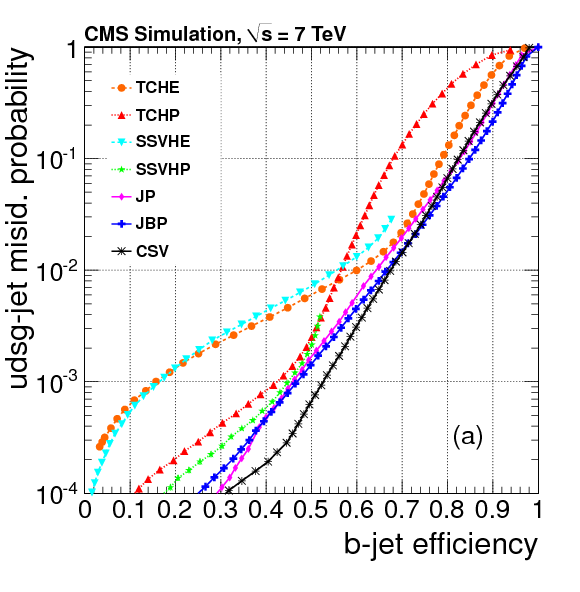
\includegraphics[width=0.49\textwidth]{figures/figAlgo_Combined_udsgvsb_Efficienies.png} &
    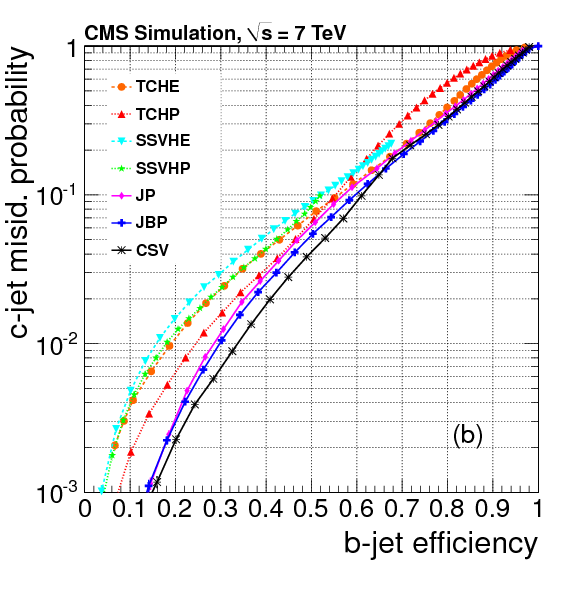
\includegraphics[width=0.49\textwidth]{figures/figAlgo_Combined_cvsb_Efficienies.png} 
  \end{tabular}
  \caption{Performance curves obtained from simulation for the algorithms described in the text. (a) light-parton and (b) c-jet misidentification probabilities as a function of the b-jet efficiency. Taken from~\cite{Chatrchyan:2012jua}.}
  \label{fig:btagging}
\end{figure}  
In order to determine the quality of a particular b-tagging algorithm, typically the misidentification probability as a function of the b-jet efficiency is compared for various taggers. Such a performance comparison is illustrated in Fig.~\ref{fig:btagging} for the tagging algorithms described above. The misidentification probability is derived separately for light-flavour and gluon initiated jets as well as c jets. The curves are derived from simulated multijet events using jets with $\pt > 60$\,\gev. For loose working points, the b-jet efficiency is around $\approx 80-85\%$, and the JBP algorithm shows the best performance. In case of medium and tight working points, the b-tag efficiency drops to $\approx 45-55\%$ and the CSV algorithm performs best. B-tagging algorithms used for analyses of data obtained at $\sqrt{s} = 8$\tev in 2012 were the TCHP, JP and CSV algorithms~\cite{CMS-PAS-BTV-13-001}. 
%In order to compare the b-tagging performance in data and simulation, two different event samples are defined. On the one hand, an inclusive multijet sample is selected while on the other hand, a sample dominated by top-pair production is extracted. These samples allow to compare quantities relevant for b tagging in data and simulation, \eg the number of secondary vertices or b-tag discriminator values. In general, input variables for b tagging show a good agreement between data and simulation with deviations within 20\%. Typically, efficiencies and misidentification probabilities are measured as function of jet transverse momentum and pseudorapidity. Any disagreement between data and simulation in terms of efficiency can be expressed as \textit{scale factors} and corrected for in analyses such that b-tagging efficiency and misidentification probability in data and simulation match. 

\section{Identification of Boosted t-Quark Jets }
\label{sec:boosted_tops}
Supersymmetric models or other scenarios describing physics beyond the standard model predict the extistence of new massive particles. Often, the coupling of these particles especially to quarks belonging to the third generation is sizeable, \eg in decays of top squarks which predominantly are expected to decay into top quarks. Consequently, such processes lead to highly-energetic top quarks in the final state which can be identified exploiting the specific properties of the top quark. 
\begin{figure}[!tp]
  \centering 
  \begin{tabular}{c}
    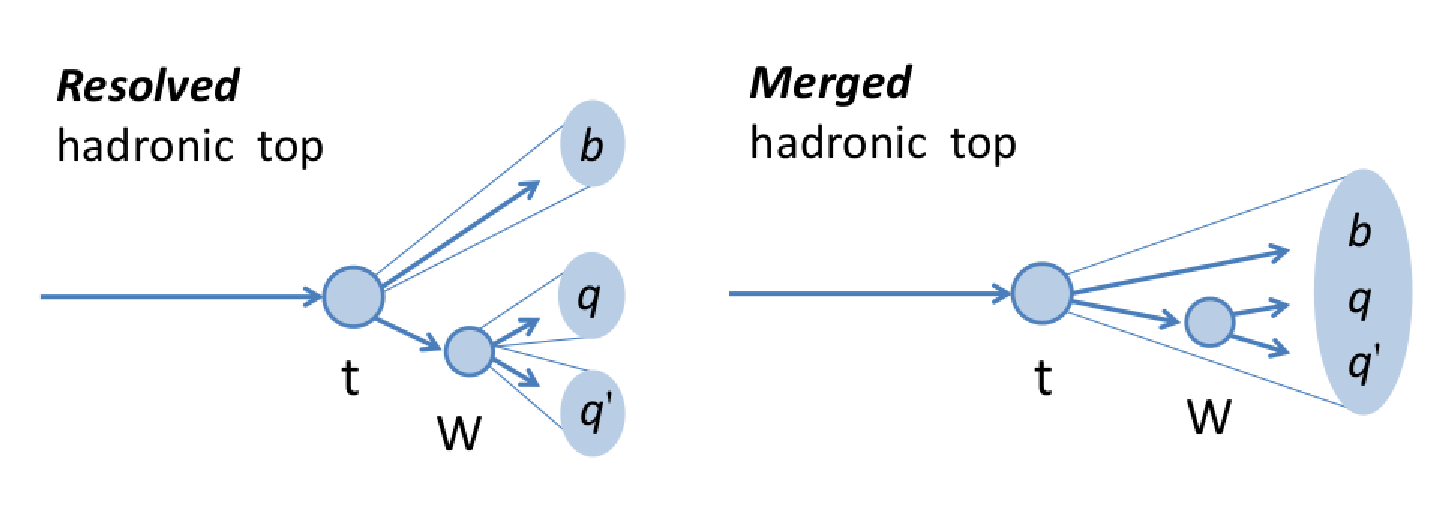
\includegraphics[width=1.0\textwidth]{figures/BoostedTops2.pdf} 
  \end{tabular}
  \caption{Schematic diagrams of the decay of a top-quark in the resolved case (\textit{left}) and the boosted scenario (\textit{right}).}
  \label{fig:boosted_top}
\end{figure}
\\
As discussed in Sec.~\ref{subsubsec:susy_backgrounds}, the decay of the top quark is experimentally characterized by the decay of the $W$ boson which makes two thirds of top quark decays resulting exclusively in hadrons. This decay mode is here referred to as \textit{hadronic top}. If top quarks are produced with $\pt \ll m_t$, the top quark decay products show up as distinct objects in the detector. In the case of hadronic tops, these are well separated jets. However, if the top transverse momentum is high, the decay products are \textit{boosted}, \ie they have large Lorentz boost, and thus are collimated in the forward direction. Consequently, they might overlap and merge into a single large jet (\textit{fat jet}). The opening angle of the decay products $\Delta R$ is expected to scale as
\begin{equation}
 \Delta R \approx 2\,m_{t} /\pt
 \label{eq:rule-of-thumb}
\end{equation}  
with the mass $m_t$ and the transverse momentum \pt of the decaying particle. Schematic diagrams of resolved and boosted top quark decays are illustrated in Fig.~\ref{fig:boosted_top}. \\
%The identification of boosted top-quark decays -- here restricted to hadronic tops -- is typically known as \textit{top tagging} and aims at the identification of the decay
%\begin{equation}
% t \rightarrow W + b \rightarrow qq' + b 
%\end{equation} 
%by analysing the substructure of fat jets. Typically, fat jets are clustered by the Cambrigde-Aachen algorithm with distance parameters of $R = 0.8$ (CA8 jet) or $R = 1.5$ (CA15 jets). Such large jets are often more prone to radiation in the event that is wrongly associated to the hard jet than jets with smaller radii. Such unwanted contributions often result in a degraded resolution. In order to mitigate such effects, \textit{jet grooming} techniques can be employed:
%\begin{description}
% \item \textbf{Filtering~\cite{Butterworth:2008tr}:} Jet constituents are recombined by rerunning the Cambridge-Aachen algorithm with a smaller distance parameter, \eg $R = 0.3$. With this procedure, subjets within the fat jet are identified: The filtering is performed by keeping only $n$ of the identified subjets. Thus, the dominant contribution from the hard process is captured while contamination from the underlying event or pileup is removed.
 %\item \textbf{Pruning~\cite{Ellis:2009su}:} In contrast to filtering, pruning does not attempt to find a particular number of subjets. Rather, the idea is to systematically remove soft and large angle recombinations in the jet clustering process. For the recombination of objects $i$ and $j$, two conditions are defined:
%\begin{equation*}
%z = \frac{\mathrm{min}(p_{\mathrm{T},i}, p_{\mathrm{T},j})}{|\vec{p}_{\mathrm{T},i} + \vec{p}_{\mathrm{T},j}|} < z_\mathrm{cut}
%\end{equation*}
%\begin{equation*}
%\Delta R_{i,j} > D_\mathrm{cut} = \frac{m_\mathrm{J}}{p_{\mathrm{T}, \mathrm{J}}}
%\end{equation*}
%where $m_\mathrm{J}$ and $p_{\mathrm{T}, \mathrm{J}}$ are the mass and the transverse momentum of the original fat jet, respectively. Whenever these two conditions are satistified, the recombination of objects $i$ and $j$ is not performed. Thus, the jet clustering is rerun using the initial jet constituents, but in addition employing a veto rule. For the Cambridge-Aachen algorithm $z_\mathrm{cut}$ is typically chosen to be 0.1.
% \item \textbf{Trimming~\cite{Krohn:2009th}:} Similarly to the filtering procedure, the jet trimming is based on the concept of identifying subjets within an initially clustered large jet, here called \textit{seed jet}. The constituents of this seed jet are reclustered using a jet clustering algorithm with a smaller distance parameter than for the seed jet. If 
%\begin{equation*}
%p_{\mathrm{T},i} < f_{\mathrm{cut}} \cdot \Lambda_{\mathrm{hard}} \; ,
%\end{equation*}
%the contributions from subjet $i$ to the seed jet are removed. Here, $f_{\mathrm{cut}}$ is a fixed dimensionless parameter and $\Lambda_{\mathrm{hard}}$ a scale chosen with respect to the specific kinematics of the event. While $f_{\mathrm{cut}}$ quantifies the expected hierarchy between FSR and ISR or pileup, the hard scale $\Lambda_{\mathrm{hard}}$ usually represents the transverse momentum of the seed jet or the effective mass of the event.% which is the scalar sum of the transverse momenta.
%\end{description} 
In order to identify decays of boosted hadronic top quarks, several \textit{top-tagging} algorithms (or short \textit{taggers}) are commissioned within the CMS experiment~\cite{CMS-PAS-JME-13-007, CMS-DP-2014-036}. Two of them are used within this thesis:
\begin{description}
%\begin{figure}[!tp]
%  \centering 
%  \begin{tabular}{cc}
%    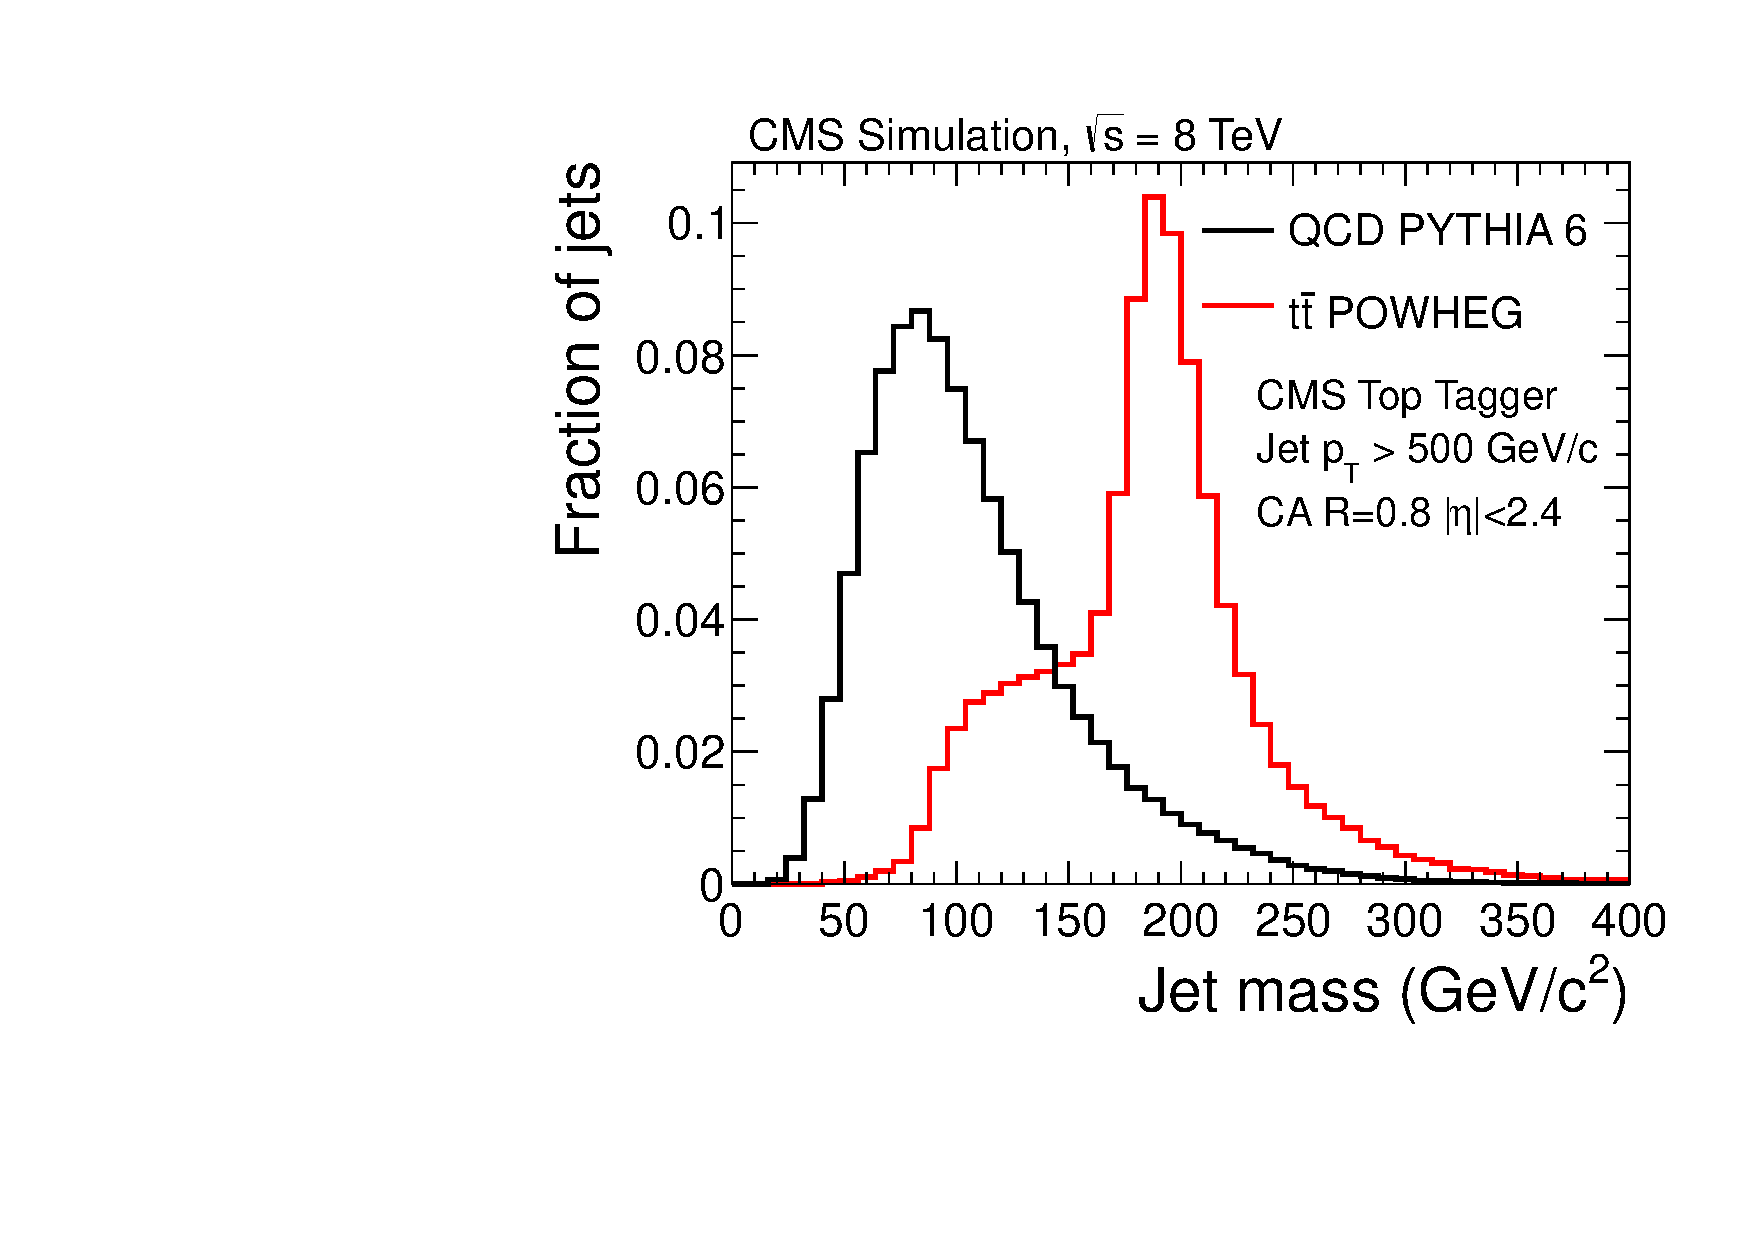
\includegraphics[width=0.49\textwidth]{figures/Draw2HistogramsFrom1File_QQ_MASS_CUT_PT_TT_MASS_CUT_PT_JetPt500.pdf} & 
%    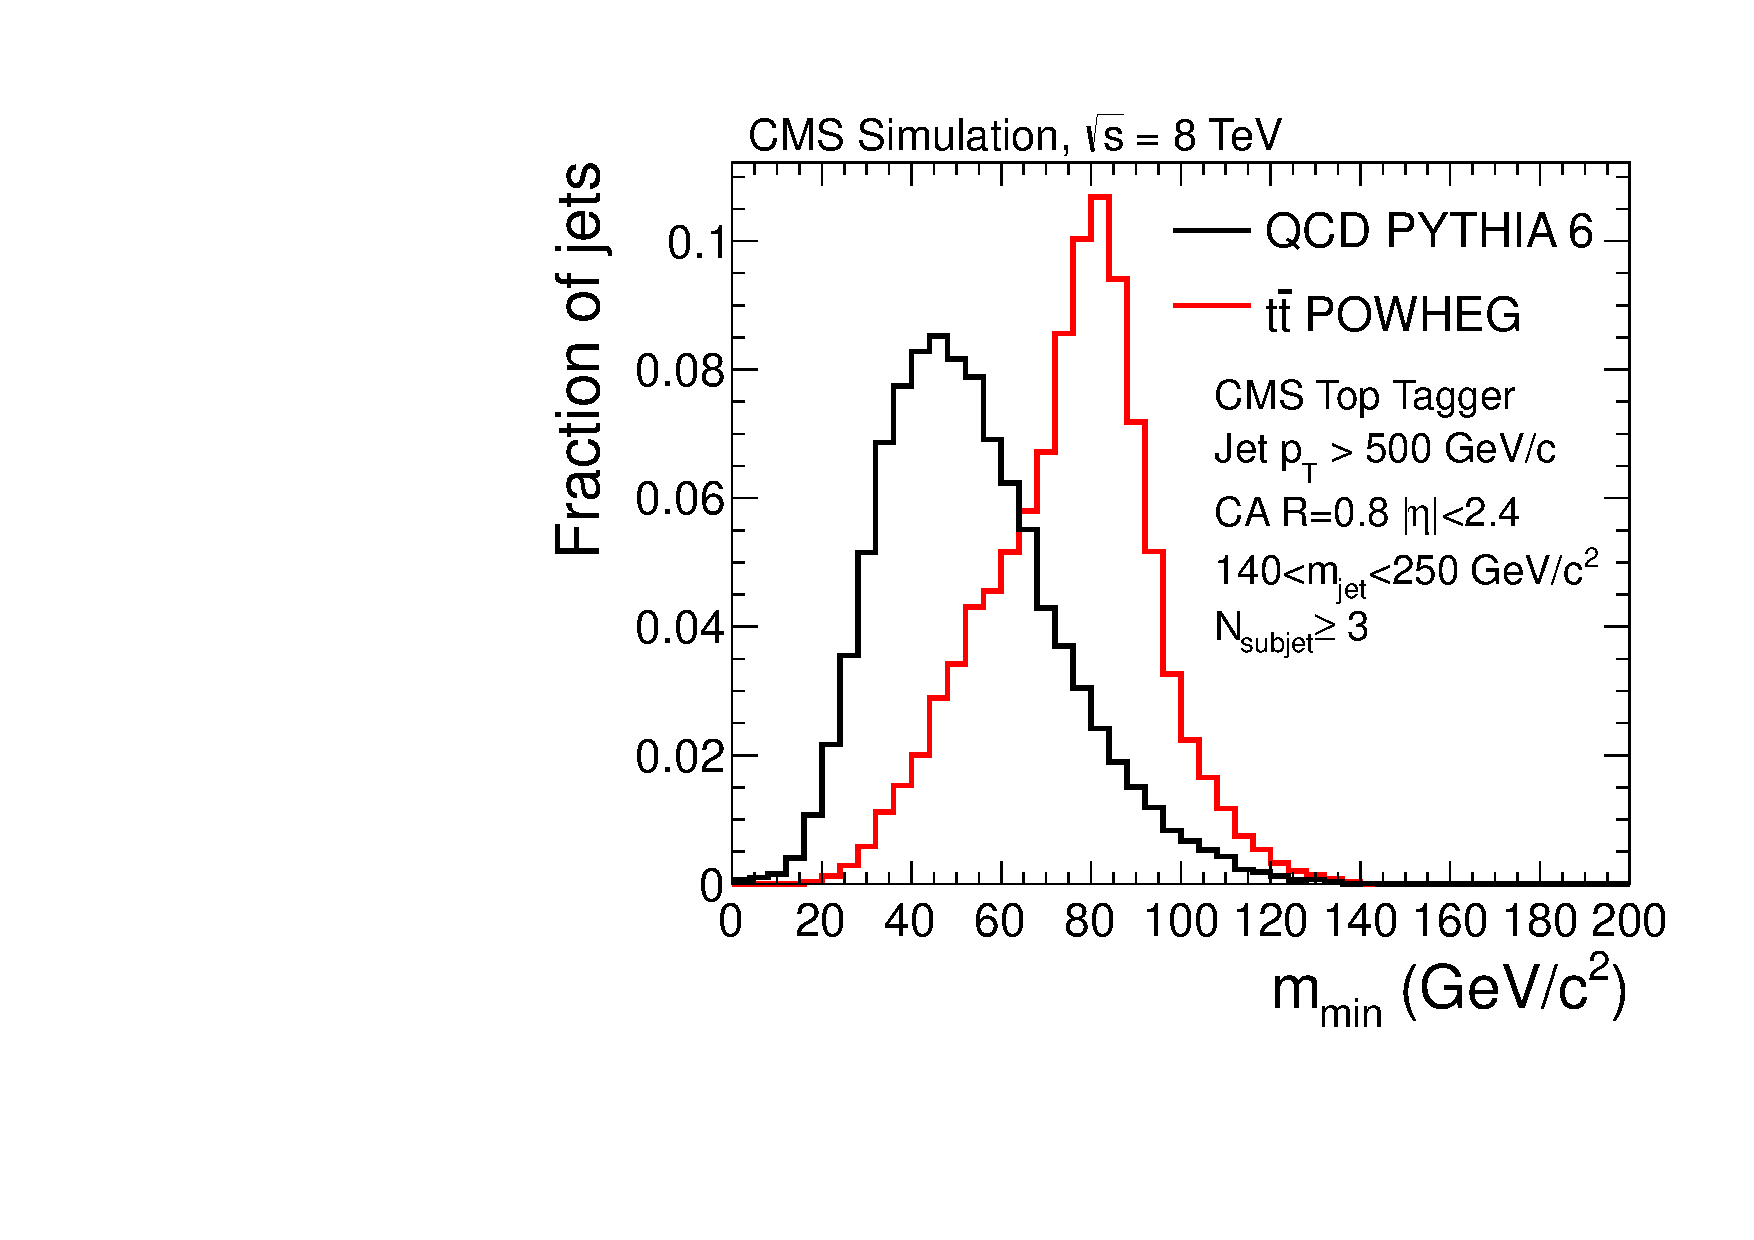
\includegraphics[width=0.49\textwidth]{figures/Draw2HistogramsFrom1File_QQ_MINM_CUT_PT_MASS_NSUB_TT_MINM_CUT_PT_MASS_NSUB_JetPt500.pdf}
%  \end{tabular}
%  \caption{Jet mass (\textit{left}) and minimum pairwise subjet mass (\textit{right}) for CA8 jets with $\pt > 500$\gev from a simulated $t\bar{t}$ \powheg sample (red) and from a simulated QCD \pythia sample (black). Taken from~\cite{CMS-PAS-JME-13-007}.}
%  \label{fig:boosted_top_cms_variables}
%\end{figure}
 \item \textbf{CMS Top Tagger:} The CMS Top Tagger~\cite{CMS-PAS-JME-09-001} is based on the top tagger developed by Kaplan et al.~\cite{Kaplan:2008ie} and acts on jets clustered by the Cambrigde-Aachen algorithm with distance parameter $R = 0.8$ (CA8 jet). These jets, used as input for the algorithm, are denoted as \textit{hard jets}. Since the decay products of the hadronic top are not expected to be all contained within one jet with $R = 0.8$ for low transverse momenta of the top quark, only jets with $\pt^\mathrm{jet} > 350$\gev are considered. In order to identify subjets within the hard jets, a two-stage decomposition procedure is applied which performs the pairwise clustering sequence used to form the hard jet in reverse order. % First, the algorithm aims at splitting the hard jet into two subclusters (\textit{primary decomposition}). Second, it is attempted to further split the clusters emerging from the first step (\textit{secondary decomposition}). 
Typically, subjets are found when they are spatially well separated and carry a significant fraction of the momentum of the hard jet. Details on the actual splitting criteria can be found in~\cite{CMS-PAS-JME-13-007}. With this approach, up to four subjets are identified within the hard jet. After a successful decomposition procedure, kinematic criteria can be applied to the identified subjets in order to tag top jets. \\
In the CMS top-tagging algorithm, as employed in this thesis, the following criteria are used:
\begin{description}
 \item -- Number of subjets $\ge$ 3
 \item -- The jet mass $m_{\mathrm{jet}}$, \ie the mass of the four-vector sum of the constituents of the hard jet, has to be close to the top-mass with $140 < m_{\mathrm{jet}} < 250$\gev.
 \item -- The invariant mass of each pair of the three subjets highest in \pt is calculated. The minimum of the pairwise masses $m_{\mathrm{min}}$ has to be $ > 50$\gev.
\end{description}
%In Fig.~\ref{fig:boosted_top_cms_variables}, the distributions for jet mass and minimum pairwise mass are illustrated for a simulated $t\bar{t}$ (red) and a QCD multijet (black) sample at $\sqrt{s} = 8$\tev. 
 \item \textbf{HEP Top Tagger:} The HEP Top Tagger~\cite{Plehn:2010st} is also based on jets clustered with the Cambrigde-Aachen algorithm, but with a larger distance parameter than the CMS Top Tagger of $R = 1.5$ (CA15 jets). This makes the HEP top-tagging algorithm especially suited for top quark decays with moderate boost and thus uses fat jets with a transverse momentum greater than 200\gev as input. %Since a larger jet size is in principle more prone to disturbing effects from the underlying event or pile-up, a sophisticated decomposition procedure is applied to distinguish hard subjets from soft components. 
Similar to the decomposition done for the CMS tagger, the identification of subjets is based on going through the cluster history of the jet in reversed order. %First, the jet is decomposed into subclusters applying a \textit{mass drop condition} discarding too soft components. Afterwards, subclusters resulting from the mass drop decomposition are reclustered into subjets and filtering criteria are applied. 
Details on the applied decomposition and reclustering criteria can be found in~\cite{CMS-PAS-JME-13-007}. In the end, the combination with the mass, determined from identified subjets, closest to the top mass is kept and reclustered to force three subjets. Kinematic selections are applied to these three final subjets in order to identify top quark decays. The following quantities are used based on the invariant mass of combinations of subjets:
%\begin{figure}[!tp]
%  \centering 
%  \begin{tabular}{cc}
%    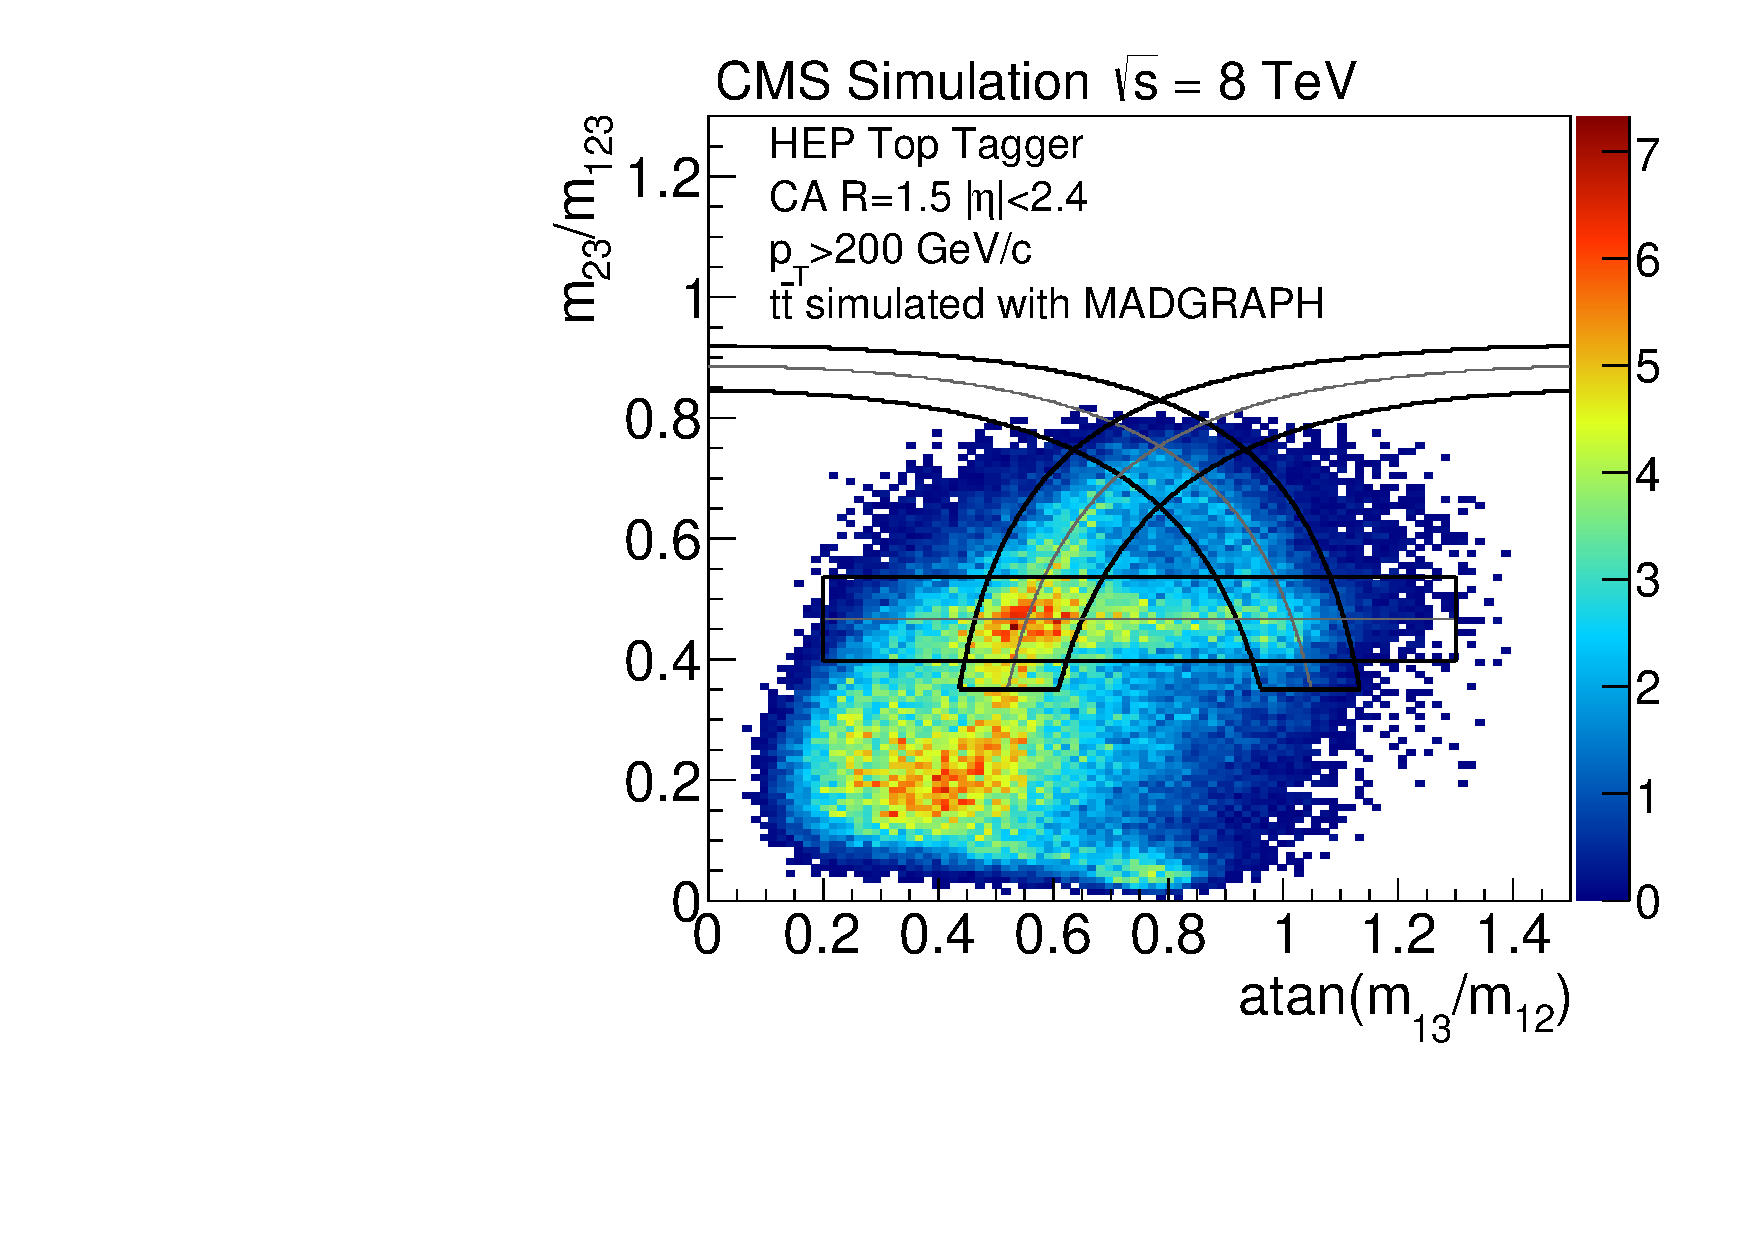
\includegraphics[width=0.49\textwidth]{figures/Pheno2DPlot_HTT2D_NOheptoptag_NOmasscut_hists_Signal_Add.pdf} & 
%    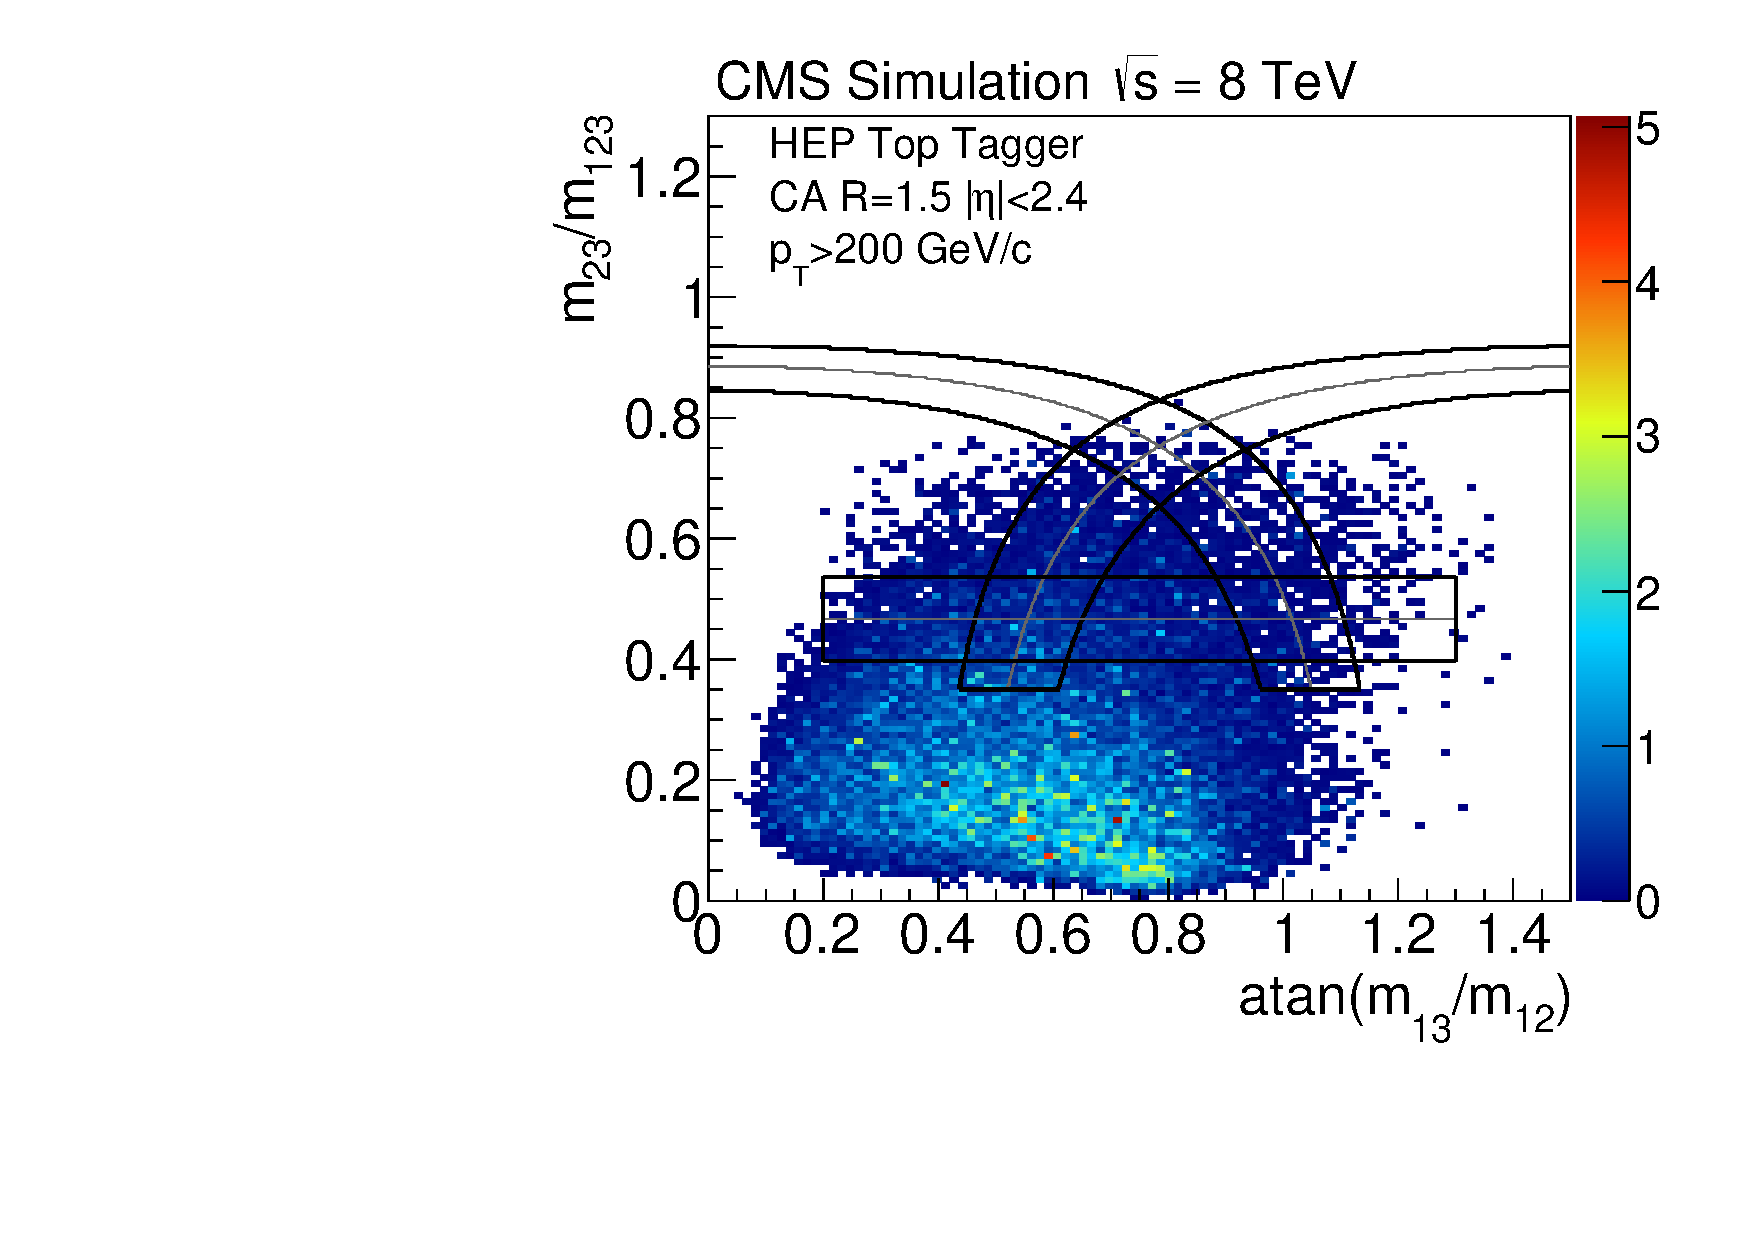
\includegraphics[width=0.49\textwidth]{figures/Pheno2DPlot_HTT2D_NOheptoptag_NOmasscut_hists_Background_Add.pdf}
%  \end{tabular}
%  \caption{Two-dimensional distributons of $m_{\mathrm{23}}/m_{\mathrm{123}}$ versus $\mathrm{atan}(m_{\mathrm{13}}/m_{\mathrm{12}})$ for HEP Top Tagger subjets from CA15 jets with $\pt > 200$\gev for a simulated $t\bar{t}$ MADGRAPH sample (\textit{left}) and for a simulated background sample composed of cross-section weighted boson + jets, diboson, single-top, $t\bar{t}$ all-hadronic and $t\bar{t}$ leptonic events (\textit{right}). The A-shaped region indicates the selected region by the HEP Top Tagger. Taken from~\cite{CMS-PAS-JME-13-007}.}
%  \label{fig:boosted_top_hep_variables}
%\end{figure}
\begin{description}
 \item -- The invariant mass of the sum of the four-vectors of the three subjets is required to be in the top mass window of $140 < m_{\mathrm{123}} < 250$\gev.
 \item -- In order to select the $W$ boson mass, the jet has to satisfy at least one of the following conditions based on the subjet pairwise masses
 \begin{equation}
0.2 < \mathrm{atan} \frac{m_{\mathrm{13}}}{m_{\mathrm{12}}} < 1.3 \; \; \mathrm{and} \; \; R_{\mathrm{min}} < \frac{m_{\mathrm{23}}}{m_{\mathrm{123}}} < R_{\mathrm{max}} 
\label{eq:hep_1}
 \end{equation}
%\end{equation}
 \begin{equation}
 R^2_{\mathrm{min}} \left( 1+ \left(\frac{m_{\mathrm{13}}}{m_{\mathrm{12}}}\right)^2 \right)  < 1 - \left( \frac{m_{\mathrm{23}}}{m_{\mathrm{123}}} \right)^2  < R^2_{\mathrm{max}} \left( 1+\left(\frac{m_{\mathrm{13}}}{m_{\mathrm{12}}} \right)^2 \right) \; \; \mathrm{and} \; \; \frac{m_{\mathrm{23}}}{m_{\mathrm{123}}} > 0.35 
\label{eq:hep_2}
\end{equation}
\begin{equation}
 R^2_{\mathrm{min}} \left( 1+ \left(\frac{m_{\mathrm{12}}}{m_{\mathrm{13}}} \right)^2 \right)  < 1 - \left(\frac{m_{\mathrm{23}}}{m_{\mathrm{123}}}\right)^2 < R^2_{\mathrm{max}}\left(1+ \left(\frac{m_{\mathrm{12}}}{m_{\mathrm{13}}} \right)^2 \right) \; \; \mathrm{and} \; \; \frac{m_{\mathrm{23}}}{m_{\mathrm{123}}} > 0.35 
\label{eq:hep_3}
\end{equation}
where the indices of $m$ indicate the rank of the considered subjets with respect to the transverse momentum, $R_{\mathrm{min}} = (1 - f_{W}) \times m_W/m_t$ and $R_{\mathrm{max}} = (1 + f_{W}) \times m_W/m_t$ for the $W$ mass width chosen to be $f_W = 0.495$.  
\end{description}
%The criteria related to the selection of the W mass are illustrated in Fig.~\ref{fig:boosted_top_hep_variables} for signal events as well as background events and indicated by the black solid lines resulting in an A-shaped region.
\end{description}
In addition, further selection criteria can be added to these taggers to achieve a potential performance improvement. These criteria are subjet-b tagging, as introduced in~\cite{CMS-PAS-BTV-13-001}, and selections on the \textit{n-subjettiness} ratio $\tau_3/\tau_2$~\cite{Thaler:2010tr, Thaler:2011gf} that denotes how likely a fat jet is composed of three subjets rather than two. \\
In analogy to the b-tagging algorithms, different working points for each top tagger can be defined characterized by a specific top-tagging efficiency and misidentification rate. Typically, the working points are chosen such that they have a minimum mistag rate for a given signal efficiency. The performance of various taggers is compared by determining the top-tagging efficiency versus the misidentification rate. Commonly, the top-tagging efficiency for simulated events is defined as the number of jets passing the top-tagging selection divided by the number of jets associated to a simulated hadronic top or anti-top passing a certain \pt selection. Similarly, the mistag rate is defined as the number of jets passing the top-tagging selection divided by the number of jets associated to a simulated quark or gluon from the hard process passing the \pt selection. In Fig.~\ref{fig:boosted_top_roc}, the mistag rate versus the top-tagging efficiency is illustrated for various taggers and parton momenta.
\begin{figure}[!t] 
  \centering 
  \begin{tabular}{c}
    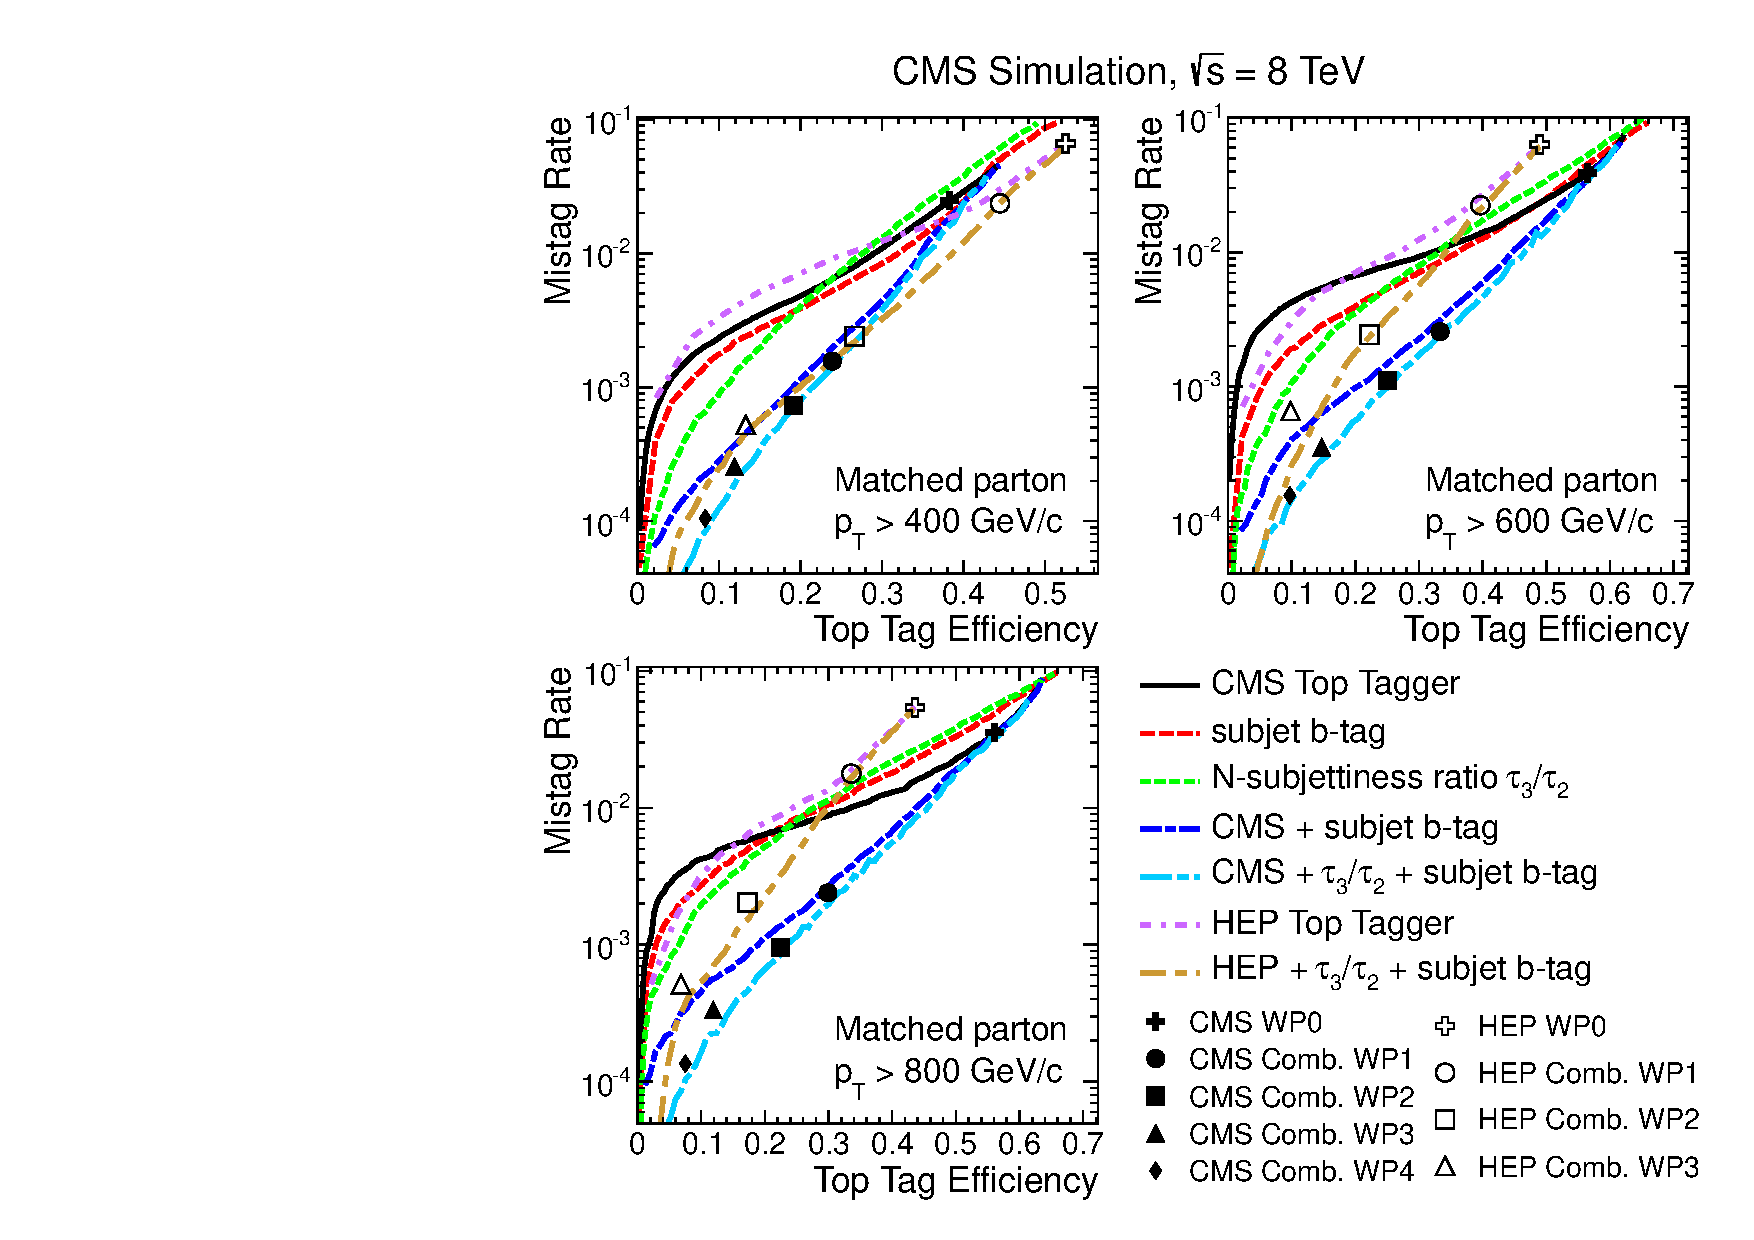
\includegraphics[width=0.8\textwidth]{figures/TopTag_ROC_Curves.pdf}  
  \end{tabular}
  \caption{Mistag rate versus top-tagging efficiency as measured from QCD \textsc{Pythia6} and \powheg \ttbar simulated events, respectively. In the cases where a jet mass cut is applied, the cut is not varied, but fixed at $140 < m_\mathrm{jet} < 250$\gev. N-subjettiness is calculated using $R = 0.8$ jets except when used in combination with the HEP Top Tagger in which case $R = 1.5$ jets are used. Signal jets are matched to simulated hadronic generated top quarks, while background jets are matched to simulated partons from the hard scatter. Distributions are shown for three \pt selections, where the \pt cut is applied to the matched generated parton~\cite{CMS-PAS-JME-13-007}.}
  \label{fig:boosted_top_roc}
\end{figure}
The top-tagging efficiency determined from simulated $t\bar{t}$ events for the selection criteria described above amounts to 35.3\% for a matched parton-\pt of $> 200$\gev for the HEP Top Tagger (HEP WP0) and 38.3\% for a matched parton-\pt of $> 400$\gev for the CMS Top Tagger (CMS WP0) while the mistag rates, as determined from simulated QCD multijet events, are 2.6\% and 2.5\%, respectively. However, the tagging performance shows a moderate dependence on pileup such that in high pileup environments a performance degradation is expected. For instance, in the case of the CMS Top Tagger %the efficiency stays rather stable as a function of the number of primary vertices with a slope of $0.031\% \pm 0.034\%$ while 
the mistag rate increases with a slope of $0.095\% \pm 0.006\%$ as a function of the number of primary vertices.       

%\subsection{Subjet B-Tagging}
%\label{sec:boosted_tops_subjet_b}

%\subsection{N-subjettiness}
%\label{sec:boosted_tops_n_subjettiness}
